\documentclass[final,12pt,nopreprintline,longtitle]{elsarticle}

\usepackage{amssymb}
\usepackage{amsmath}
\usepackage{lineno}
\usepackage{xurl}
\usepackage[hidelinks]{hyperref}
\usepackage{cleveref}
\usepackage{geometry}
\usepackage{enumitem}
\usepackage{caption}
\usepackage{booktabs}
\usepackage{graphicx}
\usepackage{microtype}
\usepackage{tikz}
\usepackage{float}
\usepackage[section]{placeins}
\usepackage{paracol}

\newcommand{\paperinput}[1]{\input{#1}}
\newcommand{\paperbibliography}[1]{\bibliography{#1}}

\journal{Computer Physics Communications}

\renewcommand{\v}{\mathbf{v}}
\newcommand{\V}{\mathbf{V}}
\newcommand{\x}{\mathbf{x}}
\renewcommand{\k}{\mathbf{k}}
\newcommand{\h}{\boldsymbol{h}}
\newcommand{\kvec}{\mathbf{k}}
\newcommand{\hvec}{\boldsymbol{h}}
\newcommand{\Sf}{\mathbf{S}_f}
\newcommand{\Tzero}{\mathbf{T}_0}
\newcommand{\Tone}{\mathbf{T}_1}
\newcommand{\betaac}{\beta}
\newcommand{\plotAidDisclosure}{Plotting code was prepared with assistance from
OpenAI Codex (model \texttt{gpt-6-astra}); see \cref{sec:aiWorkflow}.}
\newcommand{\schematicAidDisclosure}{Drawing code was prepared with assistance from
OpenAI Codex (model \texttt{gpt-6-astra}).}
\newcommand{\plotAidDisclosureRevision}{Plotting code was prepared with assistance
from Claude Code (Anthropic, model \texttt{claude-opus-5-5}); see
\cref{sec:aiWorkflow}.}
\newcommand{\schematicAidDisclosureRevision}{Drawing code was prepared with
assistance from Claude Code (Anthropic, model \texttt{claude-opus-5-5}).}

\makeatletter
\def\ps@pprintTitle{%
    \let\@oddhead\@empty
    \let\@evenhead\@empty
    \let\@oddfoot\@empty
    \let\@evenfoot\@empty}
\makeatother

\widowpenalty=10000
\clubpenalty=10000

\begin{document}

\begin{frontmatter}

\title{An unstructured finite-volume Helmholtz method with perfectly matched layers for heterogeneous two-phase acoustics}

\author[mma]{Chuanchao Xu}
\ead{xu@mma.tu-darmstadt.de}
\author[mma]{Jun Liu}
\author[must]{Jan Helge Dörsam}
\author[must]{Mario Kupnik}
\author[mma]{Tomislav Mari\'{c}\texorpdfstring{\corref{cor1}}{}}
\ead{maric@mma.tu-darmstadt.de}
\author[mma]{Dieter~Bothe}
\ead{bothe@mma.tu-darmstadt.de}
\cortext[cor1]{Corresponding author.}

\affiliation[mma]{organization={Mathematical Modeling and Analysis,
    Mathematics Department, TU Darmstadt},
    addressline={Peter-Gruenberg-Strasse 10},
    city={Darmstadt}, postcode={64287},
    country={Germany}}
\affiliation[must]{organization={Measurement and Sensor Technology,
    Department of Electrical Engineering and Information Technology,
    TU Darmstadt},
    addressline={Merckstrasse 25},
    city={Darmstadt}, postcode={64283},
    country={Germany}}

\begin{abstract}
\small
Acoustic levitation and manipulation of liquid drops require the sound field
around a drop of given shape inside a device that radiates into open space.
We present a cell-centred finite-volume method for the heterogeneous Helmholtz
equation that takes fixed drop interfaces from a volume-of-fluid (VOF) field
on an unstructured mesh and truncates the domain with perfectly matched layers
(PMLs).  Because the drop enters only through its volume-fraction field, the
acoustic response of different drop shapes is computed on the same mesh
without remeshing, which makes the method suited for coupling with VOF
simulations of drop motion in acoustic levitators.  The pressure converges at
second order for homogeneous waves on the tested orthogonal and
non-orthogonal meshes, for a layered gas--liquid--PML case and for
baffled-piston radiation.  A penetrable sphere truncated by the PML converges
as with exact boundary data: at second order for an oil drop in water, and at
about first order for a water drop in air, where the density ratio is about
800.  Radiation forces on sound-hard spheres differ from the Gorkov limit by
less than $1.5\%$ over the tested radius range, and a levitator height sweep
shows how the reflector force depends on the drop shape.
\end{abstract}

\begin{keyword}
Helmholtz equation \sep unstructured FVM \sep heterogeneous acoustics
\sep two-phase media \sep volume fraction \sep perfectly matched layer
\end{keyword}

\end{frontmatter}

\linenumbers

\section{Introduction}
\label{sec:intro}

Acoustic levitation suspends liquid drops without mechanical contact by means
of the acoustic radiation force.  Predicting the acoustic loading requires the
pressure and velocity fields in the device, including the field scattered by
the sample.  A liquid drop is therefore part of the acoustic system: its
geometry and material properties affect reflection and transmission, which in
turn change the sound field and the forces acting on the device and sample.
Numerical models of levitation must account for this interaction rather than
prescribe an incident standing wave independently of the inclusion
\cite{andrade2019numerical}, in particular when the size of the inclusion is
comparable to the acoustic wavelength.

For excitation at a prescribed frequency, a time-harmonic formulation computes
the linear acoustic response without resolving individual acoustic periods.
The complex pressure amplitude is obtained from the resulting Helmholtz
equation, and the acoustic radiation force is computed from this amplitude.
The density and compressibility of the medium enter the Helmholtz equation as
coefficients.  In gas--liquid systems, these properties change sharply across
the interface, and their contrasts determine how sound is reflected and
transmitted.  Device boundaries introduce further geometrical constraints,
while radiation into the surroundings requires a finite computational domain
to represent an open physical system.  The numerical problem thus combines
material discontinuities, geometry and domain truncation.

For domain truncation, a perfectly matched layer (PML) extends the physical
domain by an absorbing region that, in the continuous formulation, admits and
attenuates outgoing waves without reflection.  PMLs for the
Helmholtz equation have been studied in finite-element formulations
\cite{Harari2000,Bermudez2007}, and Kaltenbacher et al.\ proposed a modified
PML formulation for time-domain acoustic waves
\cite{Kaltenbacher2013modified}.  The present work adopts the latter in
time-harmonic form and implements it within an unstructured finite-volume
framework.

Existing levitation models account for the effect of a sample on the acoustic
response.  Yarin et al.\ \cite{yarin1998acoustic} computed the field
scattered by an axisymmetric drop with a boundary-element method and coupled
the acoustic radiation pressure to the calculation of steady drop shapes; the
incident field was prescribed as the standing wave of an infinitely long
levitator.  Later finite-element models also represented the device geometry.
Bänsch and Götz \cite{bansch2018numerical} computed the drop position and shape
together with acoustic streaming and evaporation in a closed levitator with
transducer and reflector geometry, and Andrade and Marzo
\cite{andrade2019numerical} used an axisymmetric acoustic model with a PML
for domain truncation and coupled the acoustic loading to a Young--Laplace
calculation of drop equilibrium.  These models treat the drop interface as a
sound-hard boundary with zero normal acoustic velocity, on the basis of the
large air--water impedance contrast.  This
treatment cannot be applied to media of comparable acoustic impedance, such
as water and oil.  In general, the numerical problem outlined above must
therefore be solved with a method that resolves the interface between the two
media.

In unstructured finite-volume methods, a cell-centred volume fraction is
widely used to represent different media, as in geometric volume-of-fluid
(VOF) methods.  For a water drop in air, the volume fraction describes the
drop geometry: each cell stores the fraction of its volume occupied by water,
and the interface within partially filled cells can be reconstructed
geometrically from the volume fractions of the cell and its neighbours.  With
this two-phase representation, the discretized Helmholtz equation can be
solved over the entire physical domain containing both media.  An important
consequence is that different drop geometries require no remeshing, because
the interface need not coincide with mesh faces.  The same mesh can therefore
be used in geometric sweeps that vary the inclusion shape.  This also makes
the method a natural
building block for simulating drop motion and deformation in acoustic
levitators, where the acoustic field must be recomputed after every update of
the drop shape.

Helmholtz solvers for complex geometries have established precedents in other
acoustic applications.  Nicoud et al.\ developed a finite-element solver on
unstructured meshes for thermoacoustic modes with complex boundary impedances
and flame coupling \cite{Nicoud2007}, and Long et al.\ developed a
finite-volume method for the Helmholtz equation in coastal-ocean environments
\cite{Long2015}.  These studies establish treatments of acoustic propagation
and geometrical constraints in their respective settings.  The requirement considered here is
more specific: acoustic fluxes and material coefficients must be constructed
from a gas--liquid volume fraction on a cell-centred polyhedral mesh and used
together with open-domain truncation.

Specialized interface methods provide other ways to treat discontinuous
acoustic coefficients.  Zhang and LeVeque incorporated jump conditions into a
Cartesian immersed-interface method for time-domain acoustics
\cite{ZhangLeVeque1997}, and Baruch et al.\ constructed high-order
one-dimensional schemes for time-harmonic equations with discontinuous
coefficients \cite{Baruch2009}.  Jeong et al.\ enforce the interface
conditions for reflection and transmission using ghost points on a Cartesian
volume grid and an unstructured surface description of the interface
\cite{Jeong2021}.  These methods impose the interface conditions through
modified stencils or ghost points.  In the present formulation, the standard
finite-volume stencil is retained, and the interface enters the acoustic
operator only through the material coefficients of cells and faces, which are
computed from the volume fraction and the reconstructed interface.

The geometric information required for these coefficients, namely the
reconstructed interface in partially filled cells and the liquid-covered area
of each face, is provided on general meshes by geometric VOF methods such as
isoAdvector and the reconstructed distance-function PLIC method
\cite{Roenby2016,Scheufler2019}.  These methods were developed for interface
reconstruction and advection in two-phase flow; here, their geometric operations are used to construct the
acoustic fluxes.

This paper develops a cell-centred Helmholtz--PML discretization for
heterogeneous gas--liquid media in which the volume fraction defines the cell
coefficients and the reconstructed interfaces define shared face fractions.
The verification examines pressure and velocity, transmission, PML
truncation, scattering by penetrable spheres, baffled-piston radiation and
radiation forces, and a
levitator height sweep demonstrates the calculation of a device response for
different drop shapes.

The model assumes linear, inviscid, adiabatic acoustics about a quiescent base
state.  The interface is fixed during each solve.  Mean flow,
dissipative losses, nonlinear wave propagation and interface evolution are
outside this scope.  The companion software preprint
\cite{Xu2026AcousticHelmholtzFoam} documents the program architecture, case
interface, distributed assembly, installation, tests and performance.  The
present paper develops the numerical formulation and assesses its accuracy
and physical use.

\Cref{sec:model} presents the model and PML formulation, and
\cref{sec:discretization} derives the finite-volume discretization and outlines
its implementation.  \Cref{sec:verification} presents the reference studies,
\cref{sec:application} the levitator application, and
\cref{sec:discussion,sec:conclusions} the implications, limitations and
conclusions.

\section{Mathematical model}
\label{sec:model}

\subsection{Wave equation for heterogeneous media}
The linear acoustic derivation shows how the spatially varying density
enters the conservative pressure equation and fixes the time convention used
in the Helmholtz, PML and finite-volume formulations.
The governing equations of fluid motion for density $\rho$, pressure $p$, and velocity $\v$ are expressed as follows:
\begin{itemize}
\item Mass conservation
        \begin{equation}
            \frac{\partial \rho}{\partial t} + \nabla\cdot(\rho \v)=0.
            \label{eq:massConserv}
        \end{equation}
        \item Momentum conservation, neglecting gravity and viscosity
        \begin{equation}
            \frac{\partial \rho \v}{\partial t} + \nabla\cdot(\rho \v\v)=-\nabla p.
            \label{eq:momConserv}
        \end{equation}
\end{itemize}

\begin{samepage}
Consider a quiescent base state that is stationary but spatially heterogeneous,
with $\v_0=\mathbf{0}$, $\rho_0=\rho_0(\x)$,
$c=c(\x)$, and $p_0=p_0(\x)$.  All base-state fields are independent of time.
Classical perturbation theory represents the acoustic field by the first-order
quantities $\rho_1$, $p_1$, and $\v_1$, with
$|\rho_1|\ll\rho_0$ and $|p_1|\ll|p_0|$.  The fields are decomposed as
    \begin{equation}
        \begin{aligned}
            \rho(\x,t) &= \rho_0(\x) + \rho_1(\x,t), \\
            p(\x,t) &= p_0(\x) + p_1(\x,t), \\
            \v(\x,t) &= \v_1(\x,t).
            \label{eq:1stPert}
        \end{aligned}
    \end{equation}
\end{samepage}

At zeroth order, \cref{eq:momConserv} gives $\nabla p_0=0$ within each
bulk region.  Thus, $p_0$ is constant there, whereas the material fields
$\rho_0(\x)$ and $c(\x)$ may still vary spatially.

Substituting \cref{eq:1stPert} into \cref{eq:momConserv} and neglecting higher-order terms (e.g., $\rho_1\v_1$, $\v_1\v_1$) yields
        \begin{equation}
            \rho_0 \frac{\partial \v_1}{\partial t}=-\nabla p_1.
            \label{eq:1stMomConserv}
        \end{equation}

After introducing the total derivative $\frac{d}{dt}:=\frac{\partial}{\partial t} + \v \cdot \nabla$, \cref{eq:massConserv} can be written as
\begin{equation}
    \frac{d \rho}{dt} + \rho \nabla\cdot\v =0.
\end{equation}

Sound propagation is modelled as adiabatic, so $\frac{d s}{d t}=0$, where $s$
is the specific entropy, and we have \cite{LandauLifshitz1987}
\begin{equation}
     \frac{d \rho}{dt}
     =\left(\frac{\partial \rho}{\partial p}\right)_s\frac{d p}{d t}
     +\left(\frac{\partial \rho}{\partial s}\right)_p\frac{d s}{d t}
     =\frac{1}{c^2}\frac{d p}{d t}
     =\frac{1}{c^2}\left(\frac{\partial p}{\partial t}+(\v\cdot\nabla)p\right),
\end{equation}
where we have used the isentropic sound speed
$c:=\sqrt{(\partial p/\partial \rho)_s}$, evaluated locally at the base state.
The mass conservation equation
now becomes
\begin{equation}
    \frac{\partial p}{\partial t} + (\v\cdot\nabla)p + \rho c^2 \, \nabla\cdot\v = 0.
    \label{eq:pMassConti}
\end{equation}

Following the same procedure, we use the first-order perturbation ansatz \cref{eq:1stPert}. Neglecting higher-order terms gives
\begin{equation}
    \frac{\partial p_1}{\partial t} = -\rho_0 c^2\, \nabla \cdot \v_1.
    \label{eq:1stMassConserv}
\end{equation}
Taking the time derivative and then using \cref{eq:1stMomConserv} to eliminate $\v_1$ gives
\begin{equation}
    \frac{1}{\rho_0(\x)c^2(\x)}
    \frac{\partial^2p_1}{\partial t^2}
    -\nabla\cdot\left(\frac{1}{\rho_0(\x)}\nabla p_1\right)=0,
    \label{eq:heteWaveP}
\end{equation}
which is the pressure wave equation for a heterogeneous medium.  Both
coefficients retain their spatial dependence.  Taking $\rho_0$ and $c$ as
constants gives the familiar homogeneous wave equation
\begin{equation}
    \frac{\partial^2 p_1}{\partial t^2} = c^2 \Delta p_1.
\end{equation}

\subsection{Helmholtz equation}
For a linear acoustic system driven at a single angular frequency, the
steady response after transients have decayed can be written in the following
time-harmonic form \cite{morse1986theoretical}
\begin{equation}
    \begin{aligned}
        p_1(\x,t) &= \mathrm{Re}(e^{-i\omega t}P(\x)),\\
        \v_1(\x,t) &= \mathrm{Re}(e^{-i\omega t}\V(\x)).
    \end{aligned}
    \label{as:timeHarmonic}
\end{equation}
where the complex pressure
$P(\x)=P_{re}(\x)+iP_{im}(\x)$ is a spatial function.
Inserting \cref{as:timeHarmonic} into the first-order momentum
equation~\eqref{eq:1stMomConserv} gives
\begin{equation}
    i\omega\rho_0 \V = \nabla P,
    \label{eq:velocityComplex}
\end{equation}
or equivalently $\V=\nabla P/(i\omega\rho_0)$.  Thus,
$\V_{re}=\nabla P_{im}/(\omega\rho_0)$ and
$\V_{im}=-\nabla P_{re}/(\omega\rho_0)$.
Substituting \cref{as:timeHarmonic} into the general wave
equation~\eqref{eq:heteWaveP} then gives
\begin{equation}
    \nabla\cdot\bigl(a(\x)\nabla P\bigr)
    +\omega^2\betaac(\x)P=0,
    \qquad
    a(\x):=\frac{1}{\rho_0(\x)},\quad
    \betaac(\x):=\frac{1}{\rho_0(\x)c^2(\x)}.
    \label{eq:heteHelmholtz}
\end{equation}
Equivalently, multiplication by $\rho_0$ gives
$\rho_0\nabla\cdot(\nabla P/\rho_0)+k^2P=0$, where the local wavenumber is
$k(\x)=\omega/c(\x)$.

\paragraph{Sharp two-phase special case}
Equation~\eqref{eq:heteHelmholtz} describes a generally heterogeneous medium.
For a sharp gas--liquid interface $\Gamma$, its conservative form is
interpreted weakly over the complete domain, with the piecewise-constant
coefficients
\begin{equation}
    \rho_0=\chi_l\rho_l+(1-\chi_l)\rho_g,
    \qquad
    a:=\frac{1}{\rho_0},
    \qquad
    \betaac:=\frac{1}{\rho_0c^2}
      =\frac{\chi_l}{\rho_lc_l^2}
       +\frac{1-\chi_l}{\rho_gc_g^2},
    \label{eq:sharpTwoPhaseCoefficients}
\end{equation}
where $\chi_l$ is the liquid indicator, equal to one in the liquid and zero in
the gas.  The corresponding conservative Helmholtz equation is
$\nabla\cdot(a\nabla P)+\omega^2\betaac P=0$.  The equilibrium interface
geometry is fixed during each solve, and first-order capillary--acoustic
coupling is neglected.  This is appropriate away from capillary resonances
when the resulting interfacial stress is small relative to the acoustic stress
\cite{Krechetnikov2019,ShapiroWeinstein2011}; for the planar one-dimensional
interface considered below, the curvature perturbation vanishes identically
\cite{Krechetnikov2019}.  Pressure and its normal flux then satisfy
\begin{equation}
    [P]_\Gamma=0,
    \qquad
    [a\nabla P\cdot\mathbf n_\Gamma]_\Gamma=0,
    \label{eq:interfaceJumpConditions}
\end{equation}
where $[\phi]_\Gamma=\phi_l-\phi_g$ at the interface.  Surface tension therefore determines the
equilibrium pressure jump of the base state but does not enter the present
first-order acoustic problem.  \Cref{sec:materialRepresentation} introduces
the VOF representation used to discretize these discontinuous coefficients.


\subsection{Acoustic radiation pressure}
The time-averaged force on a droplet in an acoustic levitator is obtained from
the acoustic radiation pressure. Its relation to the computed first-order
acoustic fields is summarized below.
The following derivation assumes a homogeneous medium, so the unperturbed
density $\rho_0$ and sound speed $c$ are constants rather than spatial fields.
The fields are expanded to second order as
\begin{equation}
    \begin{aligned}
        \rho(\x,t) &= \rho_0 + \rho_1(\x,t) + \rho_2(\x,t), \\
        p(\x,t) &= p_0 + p_1(\x,t) + p_2(\x,t), \\
        \v(\x,t) &= \v_1(\x,t) + \v_2(\x,t).
        \label{eq:2stPert}
    \end{aligned}
\end{equation}
Substituting this expansion into the momentum equation~\eqref{eq:momConserv},
neglecting terms above second order, and using the first-order momentum
equation~\eqref{eq:1stMomConserv} gives
\begin{equation}
    \nabla p_2 =
    -\rho_0\frac{\partial \v_2}{\partial t}
    -\frac{\partial (\rho_1\v_1)}{\partial t}
    -\rho_0\nabla\cdot(\v_1\v_1).
\end{equation}
Expanding $\partial(\rho_1\v_1)/\partial t$ and using the first-order
momentum and mass equations~\eqref{eq:1stMomConserv} and
\eqref{eq:1stMassConserv} yields
\begin{equation}
    \nabla p_2 =
    -\rho_0\frac{\partial \v_2}{\partial t}
    +\frac{\nabla p_1^2}{2c^2\rho_0}
    -\rho_0(\nabla\v_1)\cdot\v_1.
\end{equation}
Here the isentropic relation $p_1=c^2\rho_1$ has been used. For an
irrotational first-order velocity field, $\v_1=\nabla\Phi$, the identity
$(\nabla\v_1)\cdot\v_1=\frac{1}{2}\nabla|\v_1|^2$ applies. Moreover, the
time average of $\partial\v_2/\partial t$ over one driving period vanishes.
Denoting the time average by $\langle\cdot\rangle:= \frac{1}{T}\int_0^T \cdot \, dt$ therefore gives
\begin{equation}
    \langle p_2\rangle =
    \frac{\langle p_1^2\rangle}{2\rho_0c^2}
    -\frac{\rho_0}{2}\langle|\v_1|^2\rangle.
\end{equation}
Finally, applying the time-harmonic ansatz \cref{as:timeHarmonic} gives
\begin{equation}
    \langle p_2\rangle =
    \frac{\langle \mathrm{Re}(e^{-i\omega t}P(x))^2\rangle}{2\rho_0c^2}
    -\frac{\rho_0}{2}\langle|\mathrm{Re}(e^{-i\omega t}\V(x))|^2\rangle =  \frac{ |P(x)|^2}{4\rho_0c^2}
    -\frac{\rho_0}{4}|\V(x)|^2,
    \label{eq:acousticRadiationPressure}
\end{equation}
where the time-dependent terms vanish after time averaging.  Thus, the acoustic
radiation pressure $p_{\mathrm{rad}}:=\langle p_2\rangle$
can be evaluated from the first-order pressure and velocity fields.


\subsection{Perfectly matched layer}
As the computational domain must be bounded, open acoustic systems require a
domain-truncation treatment.  An absorbing or radiation boundary condition can
be effective for a known outgoing-wave structure, whereas a perfectly matched
layer (PML) is more suitable for general multidimensional radiation problems.
In the continuous formulation, a wave enters the PML without reflection and is
attenuated within the layer.  A finite, discretized PML can still produce a
small truncation error, whose parameter and resolution dependence is assessed in
\cref{sec:pmlSensitivity}.

Following the modified PML formulation of Kaltenbacher et al.
\cite{Kaltenbacher2013modified}, each real coordinate $x_j$ is extended into a
complex coordinate $\tilde{x}_j$.  For the time convention in
\cref{as:timeHarmonic}, the directional stretching factors are
\begin{equation}
    \eta_j
    =\frac{\partial\tilde{x}_j}{\partial x_j}
    =1+\frac{\sigma_j}{i\omega},
    \qquad
    \frac{\partial}{\partial\tilde{x}_j}
    =\frac{1}{\eta_j}\frac{\partial}{\partial x_j},
    \qquad j\in\{x,y,z\}.
    \label{eq:dampEtaDef}
\end{equation}
Here, $\sigma_j=0$ in the physical domain and $\sigma_j<0$ in the PML.  The
negative sign follows from the adopted $e^{-i\omega t}$ convention.  Equivalently,
$\tilde{\x}=\x+i\h(\x)$, with
$h_j(x_j)=-\omega^{-1}\int\sigma_j(x_j)\,dx_j$.  A plane wave then satisfies
\begin{equation}
    P=|P|\exp(i\k\cdot\tilde{\x})
     =|P|\exp(-\k\cdot\h)\exp(i\k\cdot\x),
    \label{eq:planeWaveDamp}
\end{equation}
so that $\k\cdot\h>0$ produces attenuation in the PML.

Applying \cref{eq:dampEtaDef} to the heterogeneous Helmholtz equation gives
\begin{equation}
    -\frac{(i\omega)^2}{c^2}P
    +\rho_0\sum_{j\in\{x,y,z\}}
    \frac{1}{\eta_j}\frac{\partial}{\partial x_j}
    \left(
        \frac{1}{\rho_0\eta_j}
        \frac{\partial P}{\partial x_j}
    \right)=0.
    \label{eq:extendedStretchHelmholz}
\end{equation}
For coordinate-wise separable stretching, meaning that each factor depends
only on its corresponding coordinate,
$\eta_x=\eta_x(x)$, $\eta_y=\eta_y(y)$, and $\eta_z=\eta_z(z)$.  Defining
\begin{equation}
    J=\eta_x\eta_y\eta_z,
    \qquad
    q_x=\frac{\eta_y\eta_z}{\eta_x},\quad
    q_y=\frac{\eta_x\eta_z}{\eta_y},\quad
    q_z=\frac{\eta_x\eta_y}{\eta_z},
    \label{eq:pmlJacobianRatios}
\end{equation}
and multiplying \cref{eq:extendedStretchHelmholz} by $J/\rho_0$ yields
\begin{equation}
    -\frac{J(i\omega)^2}{\rho_0c^2}P
    +\sum_{j\in\{x,y,z\}}
    \frac{\partial}{\partial x_j}
    \left(
        \frac{q_j}{\rho_0}
        \frac{\partial P}{\partial x_j}
    \right)=0.
    \label{eq:reformedStretchHelmholz}
\end{equation}

Material interfaces are confined to the physical solution domain.  Each PML
region is filled with the same homogeneous exterior medium present at its inner
boundary, and therefore $\rho_0$ and $c$ are constant throughout that PML
region.  Multiplication of \cref{eq:reformedStretchHelmholz} by this constant
$\rho_0$ consequently cancels the density from the PML flux.  This is why the
PML correction is written as $\nabla\cdot(\mathbf{T}_i\nabla P)$ rather than
$\rho_0\nabla\cdot(\mathbf{T}_i\nabla P/\rho_0)$.  In the physical domain,
where the material properties may be heterogeneous, $\boldsymbol{\sigma}=0$
and all PML correction coefficients vanish; the original heterogeneous
operator is retained there.

The mass and directional stretching factors can be separated into real and
imaginary parts as
\begin{equation}
\begin{aligned}
    (i\omega)^2J
    ={}&-\omega^2
       +(\sigma_x\sigma_y+\sigma_x\sigma_z+\sigma_y\sigma_z)\\
      &+i\left[
        \omega(\sigma_x+\sigma_y+\sigma_z)
        -\frac{\sigma_x\sigma_y\sigma_z}{\omega}
      \right],\\
    q_j={}&1+T_{0jj}-iT_{1jj}.
\end{aligned}
\label{eq:pmlComplexSplit}
\end{equation}
With $P=P_{re}+iP_{im}$, the coupled real-valued PML equations are therefore
\begin{equation}
\begin{aligned}
    \frac{\omega^2}{c^2}P_{re}
    +\rho_0\nabla\cdot\left(\frac{1}{\rho_0}\nabla P_{re}\right)
    -C_0P_{re}+C_1P_{im}
    +\nabla\cdot\left(\mathbf{T}_0\cdot\nabla P_{re}
                     +\mathbf{T}_1\cdot\nabla P_{im}\right)&=0,\\
    \frac{\omega^2}{c^2}P_{im}
    +\rho_0\nabla\cdot\left(\frac{1}{\rho_0}\nabla P_{im}\right)
    -C_0P_{im}-C_1P_{re}
    +\nabla\cdot\left(\mathbf{T}_0\cdot\nabla P_{im}
                     -\mathbf{T}_1\cdot\nabla P_{re}\right)&=0,
\end{aligned}
\label{eq:helmholtzPML}
\end{equation}
where $C_0$, $C_1$ and the tensor coefficients $\mathbf{T}_0$, $\mathbf{T}_1$
are defined by
\begin{paracol}{2}
      \begin{equation*}
      %\footnotesize
        \begin{aligned}
            C_0 &= \frac{\sigma_x\sigma_y + \sigma_x\sigma_z + \sigma_y\sigma_z}{c^2} \\%[1ex]
            T_{0xx} &= \frac{\sigma_x(\sigma_y+\sigma_z-\sigma_x) - \sigma_y\sigma_z}{(\omega^2 + \sigma^2_x)}, \\
            T_{0yy} &= \frac{\sigma_y(\sigma_x+\sigma_z-\sigma_y)-\sigma_x\sigma_z}{(\omega^2 + \sigma^2_y)}, \\
            T_{0zz} &= \frac{\sigma_z(\sigma_x+\sigma_y-\sigma_z)-\sigma_x\sigma_y}{(\omega^2 + \sigma^2_z)}, \\
            \mathbf{T_0} &= \begin{pmatrix}
              T_{0xx} & 0 & 0 \\
             0 &  T_{0yy} & 0 \\
             0 & 0 &  T_{0zz}
            \end{pmatrix},
        \end{aligned}
    \end{equation*}
    \switchcolumn
       \begin{equation*}
      % \footnotesize
        \begin{aligned}
            C_1 &= \frac{\omega(\sigma_x+\sigma_y+\sigma_z) - (\sigma_x\sigma_y\sigma_z)/\omega}{c^2} \\%[1ex]
            T_{1xx} &= \frac{(\sigma_x\sigma_y\sigma_z)/\omega + \omega(\sigma_y+\sigma_z-\sigma_x)}{(\omega^2 + \sigma^2_x)}, \\
            T_{1yy} &= \frac{(\sigma_x\sigma_y\sigma_z)/\omega + \omega(\sigma_x+\sigma_z-\sigma_y)}{(\omega^2 + \sigma^2_y)}, \\
            T_{1zz} &= \frac{(\sigma_x\sigma_y\sigma_z)/\omega + \omega(\sigma_x+\sigma_y-\sigma_z)}{(\omega^2 + \sigma^2_z)}, \\
            \mathbf{T_1} &= \begin{pmatrix}
              T_{1xx} & 0 & 0 \\
             0 &  T_{1yy} & 0 \\
             0 & 0 &  T_{1zz}
            \end{pmatrix}.
        \end{aligned}
    \end{equation*}
\end{paracol}

\subsubsection{PML in axisymmetric wedges}
\label{sec:wedgePML}

Axisymmetric problems are computed on wedge meshes with one cell in the
azimuthal direction.  With the symmetry axis along $y$, the Cartesian
directions $x$ and $z$ at the wedge mid-plane are the radial and azimuthal
directions, and $r=x$.  The wedge face areas grow linearly with $r$, so for
an axisymmetric field the finite-volume balance of
\cref{eq:reformedStretchHelmholz} approximates
\begin{equation}
    -\frac{J(i\omega)^2}{\rho_0c^2}P
    +\frac{1}{r}\frac{\partial}{\partial r}
    \left(\frac{r\,q_x}{\rho_0}\frac{\partial P}{\partial r}\right)
    +\frac{\partial}{\partial y}
    \left(\frac{q_y}{\rho_0}\frac{\partial P}{\partial y}\right)=0.
    \label{eq:wedgeStretchHelmholtz}
\end{equation}
A radial PML stretches the cylindrical radius to
$\tilde r=r+ih_r(r)$, with $\eta_r=\partial\tilde r/\partial r$ and $h_r$
defined from $\sigma_r$ as in \cref{eq:dampEtaDef}.  The axisymmetric
Helmholtz equation in the stretched coordinates,
\begin{equation}
    -\frac{(i\omega)^2}{c^2}P
    +\frac{\rho_0}{\eta_r\tilde r}\frac{\partial}{\partial r}
    \left(\frac{\tilde r}{\rho_0\eta_r}\frac{\partial P}{\partial r}\right)
    +\frac{\rho_0}{\eta_y}\frac{\partial}{\partial y}
    \left(\frac{1}{\rho_0\eta_y}\frac{\partial P}{\partial y}\right)=0,
    \label{eq:radialStretchHelmholtz}
\end{equation}
becomes \cref{eq:wedgeStretchHelmholtz} after multiplication by
$\eta_r\eta_y\tilde r/(\rho_0r)$, with
$J=\eta_r\eta_y\tilde r/r$, $q_x=\eta_y\tilde r/(\eta_rr)$ and
$q_y=\eta_r\tilde r/(\eta_yr)$.  These coefficients agree with
\cref{eq:pmlJacobianRatios} for $\eta_x=\eta_r$ and $\eta_z=\tilde r/r$,
that is, for the azimuthal damping
\begin{equation}
    \sigma_z(r)=\frac{1}{r}\int_0^r\sigma_x(r')\,dr'.
    \label{eq:wedgeAzimuthalStretch}
\end{equation}
It vanishes where $\sigma_x$ vanishes, so PML regions that damp only in the
axial direction are unchanged.  With $\sigma_z=0$, the layer stretches $r$
without the factor $\tilde r/r$.  It is then not matched to radially
spreading waves, and the truncation error no longer decreases under mesh
refinement (\cref{sec:spherePML}).  All wedge computations with a radial PML
in this paper use \cref{eq:wedgeAzimuthalStretch}.

\section{Unstructured FVM Discretization}
\label{sec:discretization}

The coupled equations in \cref{eq:helmholtzPML} are discretized with a
cell-centred unstructured FVM on a polyhedral mesh
\cite{Jasak1996,Moukalled2016}.  A control volume $\Omega_P$ has volume $V_P$,
centroid $\x_P$, and boundary faces $\mathcal{S}_f$.  The outward face-area
vector is $\Sf=\mathbf{n}_f|\mathcal{S}_f|$.  The standard cell-centred
control-volume geometry is summarized in
\cref{fig:standardFVMControlVolume}.

\begin{figure}[htbp]
    \centering
    \paperinput{fvm_control_volume_tikz.tex}
    \caption{Polyhedral control-volume geometry for the cell-centred FVM.
    The owner cell $\Omega_P$ has volume $V_P$ and centroid $\x_P$.
    The highlighted face $\mathcal S_f$ has centroid $\x_f$ and outward
    area vector $\Sf=|\mathcal S_f|\mathbf n_f$.  The dashed line joins
    the owner centroid to the centroid $\x_N$ of an adjacent cell, whose
    boundary is omitted for clarity.  This is a schematic projection;
    $\mathbf d_f=\x_N-\x_P$ need not be parallel to $\Sf$.
    OpenAI Codex (OpenAI, model \texttt{gpt-6-astra}) assisted with generating
    and revising the TikZ drawing code.}
    \label{fig:standardFVMControlVolume}
\end{figure}

\begin{figure}[t]
    \centering
    \resizebox{0.98\textwidth}{!}{%
    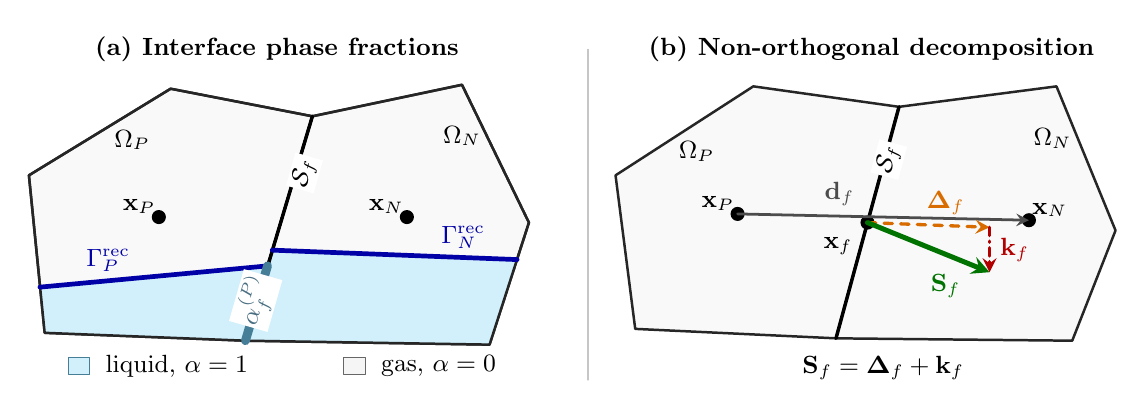
\begin{tikzpicture}[
        x=1cm,
        y=1cm,
        line cap=round,
        line join=round,
        >=stealth,
        every node/.style={font=\small},
        centre/.style={circle,fill=black,inner sep=1.8pt},
        cell/.style={draw=black!85,line width=0.9pt,fill=gray!5}
    ]
        % Panel (a): interface geometry and geometrical phase fractions.
        \begin{scope}
            \node[font=\small\bfseries] at (2.8,3.85)
                {(a) Interface phase fractions};

            \path[cell]
                (-0.15,0.25)--(2.40,0.15)--(3.25,3.00)--
                (1.45,3.35)--(-0.35,2.25)--cycle;
            \path[cell]
                (2.40,0.15)--(5.50,0.10)--(6.00,1.65)--
                (5.15,3.40)--(3.25,3.00)--cycle;

            \begin{scope}
                \clip
                    (-0.15,0.25)--(2.40,0.15)--(3.25,3.00)--
                    (1.45,3.35)--(-0.35,2.25)--cycle;
                \fill[cyan!18]
                    (-0.6,-0.2)--(6.2,-0.2)--(6.2,1.42)--
                    (2.68,1.10)--(-0.6,0.80)--cycle;
            \end{scope}
            \begin{scope}
                \clip
                    (2.40,0.15)--(5.50,0.10)--(6.00,1.65)--
                    (5.15,3.40)--(3.25,3.00)--cycle;
                \fill[cyan!18]
                    (-0.6,-0.2)--(6.2,-0.2)--(6.2,1.16)--
                    (2.74,1.30)--(-0.6,1.43)--cycle;
            \end{scope}

            % Redraw the cell boundaries over the phase fill.
            \draw[black!85,line width=0.9pt]
                (-0.15,0.25)--(2.40,0.15)--(3.25,3.00)--
                (1.45,3.35)--(-0.35,2.25)--cycle;
            \draw[black!85,line width=0.9pt]
                (2.40,0.15)--(5.50,0.10)--(6.00,1.65)--
                (5.15,3.40)--(3.25,3.00)--cycle;
            \draw[black,line width=1.25pt] (2.40,0.15)--(3.25,3.00);

            \draw[blue!65!black,line width=1.7pt]
                (-0.21,0.83)--(2.68,1.10)
                node[pos=0.30,above=-1pt] {$\Gamma_P^{\mathrm{rec}}$};
            \draw[blue!65!black,line width=1.7pt]
                (2.74,1.30)--(5.85,1.18)
                node[pos=0.78,above=-1pt] {$\Gamma_N^{\mathrm{rec}}$};
            \draw[cyan!55!black,line width=3.2pt]
                (2.40,0.15)--(2.68,1.10);

            \node[centre] at (1.30,1.72) {};
            \node[anchor=south east,inner sep=0pt,xshift=-1pt,yshift=1pt]
                at (1.30,1.72) {$\x_P$};
            \node[centre] at (4.45,1.72) {};
            \node[anchor=south east,inner sep=0pt,xshift=-1pt,yshift=1pt]
                at (4.45,1.72) {$\x_N$};
            \node at (0.96,2.70) {$\Omega_P$};
            \node at (5.15,2.75) {$\Omega_N$};
            \node[rotate=74,fill=white,inner sep=1pt] at (3.15,2.28)
                {$\mathcal S_f$};
            \node[rotate=74,fill=white,inner sep=0.8pt,
                text=cyan!45!black] at (2.53,0.66) {$\alpha_f^{(P)}$};
            \fill[cyan!18,draw=cyan!55!black] (0.15,-0.28) rectangle (0.42,-0.06);
            \node[anchor=west] at (0.50,-0.17) {liquid, $\alpha=1$};
            \fill[gray!8,draw=black!60] (3.65,-0.28) rectangle (3.92,-0.06);
            \node[anchor=west] at (4.00,-0.17) {gas, $\alpha=0$};
        \end{scope}

        % Panel divider.
        \draw[gray!45] (6.75,-0.35)--(6.75,3.85);

        % Panel (b): owner-neighbour geometry and non-orthogonal decomposition.
        \begin{scope}[xshift=7.35cm]
            \node[font=\small\bfseries] at (3.0,3.85)
                {(b) Non-orthogonal decomposition};

            \path[cell]
                (0.0,0.30)--(2.55,0.18)--(3.35,3.12)--
                (1.50,3.38)--(-0.25,2.25)--cycle;
            \path[cell]
                (2.55,0.18)--(5.55,0.15)--(6.10,1.55)--
                (5.35,3.38)--(3.35,3.12)--cycle;
            \draw[black,line width=1.25pt] (2.55,0.18)--(3.35,3.12);

            \coordinate (P) at (1.30,1.76);
            \coordinate (N) at (5.00,1.68);
            \coordinate (F) at (2.95,1.65);
            \coordinate (D) at (4.50,1.59);
            \coordinate (S) at (4.50,1.02);

            \node[centre] at (P) {};
            \node[anchor=south east,inner sep=0pt,xshift=-1pt,yshift=1pt]
                at (P) {$\x_P$};
            \node[centre] at (N) {};
            \node[anchor=south west,inner sep=0pt,xshift=1pt,yshift=1pt]
                at (N) {$\x_N$};
            \node[centre,label=below left:$\x_f$] at (F) {};
            \node at (0.78,2.55) {$\Omega_P$};
            \node at (5.3,2.72) {$\Omega_N$};
            \node[rotate=75,fill=white,inner sep=1pt] at (3.22,2.45)
                {$\mathcal S_f$};

            \draw[->,black!70,line width=1.0pt]
                (P)--(N) node[pos=0.35,above=0pt] {$\mathbf d_f$};
            \draw[->,orange!85!black,dashed,line width=1.2pt]
                (F)--(D) node[pos=0.64,above=0pt] {$\boldsymbol{\Delta}_f$};
            \draw[->,green!45!black,line width=1.8pt]
                (F)--(S) node[pos=0.64,below=3pt] {$\Sf$};
            \draw[->,red!70!black,dash dot,line width=1.2pt]
                (D)--(S) node[midway,right] {$\mathbf k_f$};
            \node[font=\small] at (3.15,-0.20)
                {$\Sf=\boldsymbol{\Delta}_f+\mathbf k_f$};
        \end{scope}
    \end{tikzpicture}%
    }
    \caption{Geometric quantities used by the cell-centred unstructured FVM.
    (a) The cell-local planar reconstructions $\Gamma_P^{\mathrm{rec}}$ and
    $\Gamma_N^{\mathrm{rec}}$ partition the adjacent cells.  The highlighted
    liquid-covered part defines the candidate $\alpha_f^{(P)}$; the shared
    fraction combines the available cuts through \cref{eq:averagedFaceFraction}.
    (b) The owner and neighbour centroids are connected
    by $\mathbf d_f$, while
    $\Sf=\boldsymbol{\Delta}_f+\mathbf k_f$ separates the orthogonal and
    non-orthogonal parts of the face-area vector.  \schematicAidDisclosure}
    \label{fig:unstructuredFVMSchematic}
\end{figure}

\subsection{Two-phase material representation}
\label{sec:materialRepresentation}

The acoustic solve accepts the volume-fraction representation used to
describe the liquid configuration, without requiring an interface-fitted
acoustic mesh.  The two-phase material field is described by a volume fraction $\alpha$, with
$\alpha=1$ in the liquid, $\alpha=0$ in the gas, and intermediate values
in interface cells.  The mesh geometry, interface reconstruction, and
non-orthogonal decomposition are summarized in
\cref{fig:unstructuredFVMSchematic}.  The one-field density and acoustic
compressibility are linearly averaged as
\begin{equation}
    \rho=\alpha\rho_l+(1-\alpha)\rho_g,
    \qquad
    \betaac
    =\alpha\betaac_l+(1-\alpha)\betaac_g,
    \qquad
    \betaac_i=\frac{1}{\rho_i c_i^2},\quad i\in\{l,g\}.
    \label{eq:materialAverages}
\end{equation}

The cell fraction is the liquid volume fraction,
\begin{equation}
    \alpha_P=\frac{1}{V_P}\int_{\Omega_P}\chi_l\,dV,
    \label{eq:geometricFractions}
\end{equation}
where $\chi_l$ is the liquid indicator.  Face fractions are evaluated from the
available adjacent-cell piecewise-linear interface constructions (PLIC), using
the geometric cutting operations of the VOF reconstruction
\cite{Roenby2016,Scheufler2019,Liu2023incons}.
For an internal face $f$ shared by cells $P$ and $N$, let
$\mathcal C_f\subseteq\{P,N\}$ contain the cells with valid reconstructed
planes.  A plane with centre $\x_{\Gamma,c}$ and unit normal $\mathbf n_c$
defines the candidate liquid half-space
\[
    H_l^{(c)}
    =\{\x:\mathbf n_c\cdot(\x-\x_{\Gamma,c})\geq 0\}.
\]
The normal is oriented towards the liquid.  Each candidate supplies its own
liquid-covered area fraction,
\begin{equation}
    \alpha_f^{(c)}
    =\frac{\displaystyle\sum_{T\in\mathcal T_f}
                |T\cap H_l^{(c)}|}
           {\displaystyle\sum_{T\in\mathcal T_f}|T|},
    \qquad c\in\mathcal C_f ,
    \label{eq:candidateFaceFraction}
\end{equation}
where $\mathcal T_f$ is a triangulation of the face; on a planar face this is
the liquid-covered area divided by the face area.

The shared face fraction is
\begin{equation}
    \alpha_f=
    \begin{cases}
        \tfrac12\bigl(\alpha_f^{(P)}+\alpha_f^{(N)}\bigr),
            & |\mathcal C_f|=2,\\
        \alpha_f^{(c)}, & \mathcal C_f=\{c\}.
    \end{cases}
    \label{eq:averagedFaceFraction}
\end{equation}
When neither cell supplies a plane, two pure cells of the same phase give the
value zero or one, and opposite pure cells separated by a mesh face use the
distance-weighted linear interpolation of $\alpha_P$ and $\alpha_N$.  On a
processor face, the plane descriptions are exchanged and the face is
triangulated in a canonical vertex order, so that both ranks form the same
average.  Face averaging thus changes only the material coefficient of the
acoustic operator, without velocity-dependent donor selection or additional
pressure unknowns.

For the face flux, the same one-field relation is adopted as a closure for
the density on faces according to
\begin{equation}
    \rho_f=\alpha_f\rho_l+(1-\alpha_f)\rho_g,
    \qquad
    a_f:=\left(\frac{1}{\rho}\right)_f=\frac{1}{\rho_f}.
    \label{eq:faceInverseDensity}
\end{equation}
The PML tensors $\mathbf{T}_{0,f}$ and
$\mathbf{T}_{1,f}$ are linearly interpolated to faces; they are smooth in the
homogeneous PML and vanish in the heterogeneous physical domain.

\subsection{Interface flux}

The transmission conditions in \cref{eq:interfaceJumpConditions} identify
$a=1/\rho$ as the coefficient of the conserved normal pressure-gradient flux.
The method retains the one-field coefficient
$a_f=1/[\alpha_f\rho_l+(1-\alpha_f)\rho_g]$ from
\cref{eq:faceInverseDensity}.  For either pressure component $Q$, the
physical-domain face contribution is
\begin{equation}
    F_f(Q)=a_f\left[
        \frac{|\Sf|^2}{\Sf\cdot\mathbf d_f}(Q_N-Q_P)
        +(\nabla Q)_f\cdot\mathbf k_f
    \right],
    \label{eq:retainedInterfaceFlux}
\end{equation}
with the geometric decomposition and corrected gradient defined below.
The first term is implicit and the nonorthogonal correction is updated
explicitly.  A common face coefficient and gradient give opposite
contributions to the adjacent unscaled conservation equations, before
multiplication by their respective cell densities.

The flux uses one coefficient on both sides of a cut face, so the interface
conditions \cref{eq:interfaceJumpConditions} are its continuum target but are
not imposed as local constraints within a cut cell.

\subsection{Control-volume balance}

For a scalar cell field $Q$, define the face flux associated with a tensor
coefficient $\mathbf{K}$ by
\begin{equation}
    \mathcal{F}_f(\mathbf{K},Q)
    :=\left(\mathbf{K}_f\cdot(\nabla Q)_f\right)\cdot\Sf.
    \label{eq:genericFaceFlux}
\end{equation}
Application of the Gauss theorem to \cref{eq:helmholtzPML} gives the two
cell balances
\begin{equation}
    (A_hP_{re})_P+(B_hP_{im})_P=0,
    \qquad
    (A_hP_{im})_P-(B_hP_{re})_P=0,
    \label{eq:discreteCellBalances}
\end{equation}
where
\begin{equation}
\begin{aligned}
    (A_hQ)_P={}&
        \rho_P\sum_{f\in\partial\Omega_P}
        a_f(\nabla Q)_f\cdot\Sf
        +\sum_{f\in\partial\Omega_P}
        \mathcal{F}_f(\mathbf{T}_0,Q)
        +(\omega^2\rho_P\betaac_P-C_{0,P})Q_PV_P,\\
    (B_hQ)_P={}&
        \sum_{f\in\partial\Omega_P}
        \mathcal{F}_f(\mathbf{T}_1,Q)
        +C_{1,P}Q_PV_P.
\end{aligned}
\label{eq:discreteOperators}
\end{equation}
The reaction coefficients and the orthogonal parts of the face fluxes are
assembled implicitly.

\subsection{Internal and boundary face gradients}

For an internal face shared by owner cell $P$ and neighbour cell $N$, let
$\mathbf{d}_f=\x_N-\x_P$.  The face-area vector is decomposed into an
orthogonal contribution $\boldsymbol{\Delta}_f$ and a non-orthogonal remainder
$\mathbf{k}_f$,
\begin{equation}
    \boldsymbol{\Delta}_f
    =\frac{|\Sf|^2}{\Sf\cdot\mathbf{d}_f}\mathbf{d}_f,
    \qquad
    \mathbf{k}_f=\Sf-\boldsymbol{\Delta}_f.
    \label{eq:faceAreaDecomposition}
\end{equation}
The corrected face-normal gradient is
\begin{equation}
    (\nabla Q)_f\cdot\Sf
    \simeq
    \frac{|\Sf|^2}{\Sf\cdot\mathbf{d}_f}(Q_N-Q_P)
    +(\nabla Q)_f\cdot\mathbf{k}_f.
    \label{eq:correctedFaceGradient}
\end{equation}
This decomposition follows the standard corrected unstructured FVM treatment
of non-orthogonal faces \cite{Jasak1996,Moukalled2016}.
Cell gradients are reconstructed with the selected unstructured gradient
scheme and interpolated linearly to the face.  The first term in
\cref{eq:correctedFaceGradient} contributes to the matrix coefficients.  When
a corrected Laplacian scheme is selected, the second term is evaluated
explicitly and updated in the non-orthogonal correction loop.  It vanishes on
an orthogonal mesh.  Tensor fluxes are evaluated from
$(\mathbf{T}_{m,f}\cdot\nabla Q_f)\cdot\Sf$ using the same face-gradient
reconstruction.

At a boundary face $b$, the flux is evaluated from the prescribed boundary
condition.  A Dirichlet condition supplies $Q_b$ and its face-normal gradient
is reconstructed from $Q_b-Q_P$, including the selected non-orthogonal
correction.  A Neumann condition directly prescribes
$g_b=\nabla Q_b\cdot\mathbf{n}_b$, giving the normal flux
$\rho_Pa_b|\mathcal{S}_b|g_b$.  In particular, a prescribed complex normal
velocity $V_n=V_{n,re}+iV_{n,im}$ gives, from the first-order momentum equation,
\begin{equation}
    \frac{\partial P_{re}}{\partial n}
    =-\omega\rho V_{n,im},
    \qquad
    \frac{\partial P_{im}}{\partial n}
    =\omega\rho V_{n,re}.
    \label{eq:velocityPressureBoundary}
\end{equation}
Here $V_n=\V\cdot\mathbf{n}$ is defined with the outward normal of the fluid
domain.  Consequently, a boundary moving into the fluid with real velocity
amplitude $u_0$ has $V_{n,re}=-u_0$ and is imposed through
$\partial P_{im}/\partial n=-\omega\rho u_0$.
For a Dirichlet condition, the coefficient multiplying the adjacent cell value
is added to the matrix diagonal, while the contribution containing the known
boundary value is transferred to the right-hand side.  Neumann data contribute
directly to the right-hand side.
Both contributions must be retained in the assembled block operator.

\subsection{Block system and correction sequence}

After assembly over all control volumes, the discrete equations have the
real-valued block form
\begin{equation}
\begin{bmatrix}
    A_h & B_h\\
    -B_h & A_h
\end{bmatrix}
\begin{bmatrix}
    \mathbf{P}_{re}\\
    \mathbf{P}_{im}
\end{bmatrix}
=
\begin{bmatrix}
    \mathbf{b}_{re}\\
    \mathbf{b}_{im}
\end{bmatrix}.
\label{eq:blockSystem}
\end{equation}
The discretization proceeds by reconstructing the interface and face fractions,
constructing the cell and face material coefficients, assembling the diagonal
and real--imaginary coupling operators, and solving \cref{eq:blockSystem}.
For a corrected non-orthogonal scheme, the explicit face-gradient correction
is refreshed and the block system is reassembled in each correction sweep.

For smooth coefficients and solutions on sufficiently regular meshes, linear
face interpolation and corrected gradients are expected to recover nominal
second-order spatial accuracy.  At a discontinuous material interface, the
accuracy also depends on the interface representation and the face coefficient
in \cref{eq:faceInverseDensity}.  Derived quantities based on reconstructed
pressure gradients can be more sensitive to mesh deformation than the primary
pressure solution.  These effects are examined in the corresponding
verification studies.

\subsection{Implementation and representative solution cost}
\label{sec:implementation}

The discretization is implemented as \texttt{acousticHelmholtzFoam} in
OpenFOAM.  Revision
\href{https://github.com/tmaric/TwoPhaseFlow/tree/7f00fc55a67aefbcfa88bdb46a4fc378bac0db0c}{\texttt{7f00fc55a67a}}
identifies the accompanying implementation
\cite{XuLiuMaric2026AcousticSoftware}.  The cell equations, including boundary
and processor-face contributions, are assembled into a distributed PETSc
matrix \cite{Balay1997}.  The default solution uses a sparse LU factorization
with MUMPS \cite{Amestoy2001}.  Each non-orthogonal correction sweep refreshes
the explicit gradient terms, reassembles the system and repeats the solve.
There are two real pressure unknowns per cell.  The utility
\texttt{setPMLFields} computes the damping field $\boldsymbol{\sigma}$,
including \cref{eq:wedgeAzimuthalStretch} on wedge meshes.  The companion
software paper
\cite{Xu2026AcousticHelmholtzFoam} describes the case inputs, assembly,
installation and execution in detail.

As a representative cost measurement, that paper reports a two-phase
levitator wedge mesh with $570\,818$ cells and $1\,141\,636$ unknowns.  On an
AMD Ryzen~7 PRO 7840U workstation with eight physical cores and
OpenFOAM-v2606, the measured elapsed time per solver invocation was
$16.36\,\mathrm{s}$ on one MPI rank and $8.71\,\mathrm{s}$ on four ranks,
after one unreported warm-up solve, excluding mesh generation, decomposition
and function-object evaluation.

\section{Verification}
\label{sec:verification}

\subsection{Computational workflow and AI assistance}
\label{sec:aiWorkflow}

During development and verification of the formulation, OpenAI Codex (OpenAI, model
\texttt{gpt-6-astra}) and Claude Code (Anthropic, model \texttt{claude-opus-5-5})  assisted with source-code changes, preparation of
verification cases, data-processing and plotting scripts, and consistency
checks between the manuscript and its supporting data.  The corresponding author directed these tasks and selected the
changes included in the implementation and the manuscript.  All numerical
results were computed with the implementation identified in
\cref{sec:implementation}.  The verification
secondary-data package records the inputs and scripts used to reproduce its
numerical plots and tables.

\subsection{Error measures}
\label{sec:errorMeasures}

For analytical references, the numerical value $y_h(\x_i)$ is compared with
$y_{\mathrm{ex}}(\x_i)$ using
\begin{equation}
    E_2 =
    \frac{\left(\sum_i w_i|y_h(\x_i)-y_{\mathrm{ex}}(\x_i)|^2\right)^{1/2}}
    {\left(\sum_i w_i|y_{\mathrm{ex}}(\x_i)|^2\right)^{1/2}}.
    \label{eq:errorMeasures}
\end{equation}
Here $w_i=V_i$ unless stated otherwise.  With $\lVert q\rVert_w^2=\sum_iw_iq_i^2$ and
$e_q=q_h-q_{\mathrm{ex}}$, the component and combined complex-pressure errors
are computed as
\begin{equation}
    E_{P_{\mathrm{re}}}
    =\frac{\lVert e_{P_{\mathrm{re}}}\rVert_w}
           {\lVert P_{\mathrm{ex},\mathrm{re}}\rVert_w},
    \qquad
    E_{P_{\mathrm{im}}}
    =\frac{\lVert e_{P_{\mathrm{im}}}\rVert_w}
           {\lVert P_{\mathrm{ex},\mathrm{im}}\rVert_w},
    \qquad
    E_P
    =\left(
      \frac{\lVert e_{P_{\mathrm{re}}}\rVert_w^2
           +\lVert e_{P_{\mathrm{im}}}\rVert_w^2}
           {\lVert P_{\mathrm{ex},\mathrm{re}}\rVert_w^2
           +\lVert P_{\mathrm{ex},\mathrm{im}}\rVert_w^2}
      \right)^{1/2}.
    \label{eq:complexPressureErrors}
\end{equation}
For two successive mesh sizes $h_1$ and $h_2$, the observed order is estimated
as
\begin{equation}
    q=\frac{\log(E_{h_1}/E_{h_2})}{\log(h_1/h_2)}.
    \label{eq:observedOrder}
\end{equation}
Six mesh levels are used for the homogeneous study, with the nominal mesh size
$h=\lambda/N_\lambda$.  The piston field is assessed on five
geometry-aligned meshes with 20--80 cells per
wavelength; the radial block boundary remains fixed at the piston edge.  For
the rigid-sphere position sweep, the force
difference is normalized by the peak
Gorkov force because a pointwise relative error is undefined at the analytical
zero-force positions.

\subsection{Homogeneous plane-wave baseline}
\label{sec:homogeneousBaseline}

The source-free baseline removes material and PML errors.  In a homogeneous
domain, the exact pressure is
\begin{equation}
    P(\x)=P_0\exp\!\left[i(\phi-\mathbf{k}\cdot\x)\right],
    \qquad |\mathbf{k}|=\omega/c_0.
    \label{eq:homogeneousPlaneWave}
\end{equation}
The domain dimensions are $L_x=1.125\, \lambda$ and
$L_y=0.625\, \lambda$, with $P_0=1\,\mathrm{Pa}$ and $\phi=\pi/6$.
The Dirichlet case uses a wave at $30^\circ$ to the $x$ axis and exact pressure
on all boundaries.  The mixed case uses an $x$-directed wave, exact pressure at
$x=0$, exact non-zero normal gradient at $x=L_x$, and zero normal gradient on
the lateral boundaries.  The exact velocity follows from
\cref{eq:velocityComplex}.  The two boundary configurations and mesh families
are summarized in \cref{fig:homogeneousBaselineSchematic}.

\begin{figure}[htbp]
    \centering
    \resizebox{0.96\textwidth}{!}{%
    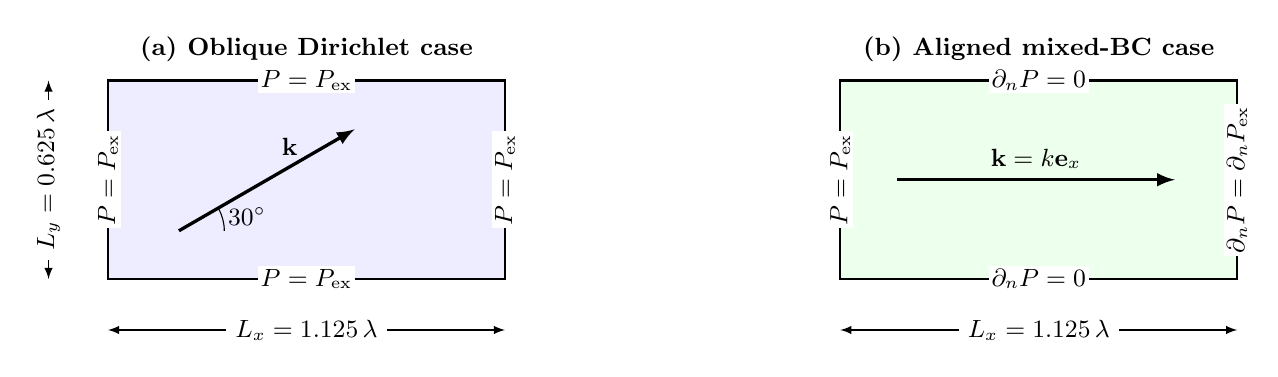
\begin{tikzpicture}[x=0.72cm,y=0.72cm,>=latex,font=\small]
        \def\w{7.0}
        \def\h{3.5}

        \begin{scope}
            \fill[blue!7] (0,0) rectangle (\w,\h);
            \draw[thick] (0,0) rectangle (\w,\h);
            \node[font=\small\bfseries] at (3.5,4.05)
                {(a) Oblique Dirichlet case};
            \node[rotate=90,fill=white,inner sep=1pt] at (0,1.75)
                {$P=P_{\mathrm{ex}}$};
            \node[rotate=90,fill=white,inner sep=1pt] at (\w,1.75)
                {$P=P_{\mathrm{ex}}$};
            \node[fill=white,inner sep=1pt] at (3.5,0)
                {$P=P_{\mathrm{ex}}$};
            \node[fill=white,inner sep=1pt] at (3.5,\h)
                {$P=P_{\mathrm{ex}}$};
            \draw[->,very thick] (1.25,0.85) -- (4.35,2.64)
                node[pos=0.63,above] {$\mathbf{k}$};
            \draw (2.05,0.85) arc[start angle=0,end angle=30,radius=0.8];
            \node at (2.45,1.10) {$30^\circ$};
            \draw[<->] (0,-0.90) -- (\w,-0.90)
                node[midway,fill=white] {$L_x=1.125\, \lambda$};
            \draw[<->] (-1.05,0) -- (-1.05,\h)
                node[midway,fill=white,rotate=90] {$L_y=0.625\, \lambda$};
        \end{scope}

        \begin{scope}[xshift=9.3cm]
            \fill[green!7] (0,0) rectangle (\w,\h);
            \draw[thick] (0,0) rectangle (\w,\h);
            \node[font=\small\bfseries] at (3.5,4.05)
                {(b) Aligned mixed-BC case};
            \node[rotate=90,fill=white,inner sep=1pt] at (0,1.75)
                {$P=P_{\mathrm{ex}}$};
            \node[rotate=90,fill=white,inner sep=1pt] at (\w,1.75)
                {$\partial_n P=\partial_n P_{\mathrm{ex}}$};
            \node[fill=white,inner sep=1pt] at (3.5,0)
                {$\partial_nP=0$};
            \node[fill=white,inner sep=1pt] at (3.5,\h)
                {$\partial_nP=0$};
            \draw[->,very thick] (1.0,1.75) -- (5.9,1.75)
                node[midway,above] {$\mathbf{k}=k\mathbf{e}_x$};
            \draw[<->] (0,-0.90) -- (\w,-0.90)
                node[midway,fill=white] {$L_x=1.125\, \lambda$};
        \end{scope}

    \end{tikzpicture}
    }
    \caption{Boundary-condition configurations for the homogeneous plane-wave
    baseline: (a) oblique propagation with exact Dirichlet data and (b) aligned
    propagation with mixed Dirichlet--Neumann data.  Each configuration is
    solved on both mesh families shown in \cref{fig:homogeneousMeshes}.  \schematicAidDisclosure}
    \label{fig:homogeneousBaselineSchematic}
\end{figure}

Two hexahedral mesh families are refined from 16 to 96 cells per wavelength.
The orthogonal family uses the orthogonal Laplacian.  In the non-orthogonal interior mesh
family, the boundary and first interior point lines remain Cartesian, giving
one orthogonal boundary-cell layer.  The deformation is ramped smoothly over
$0.15\min(L_x,L_y)$ to the prescribed interior deformation, whose amplitude
factor is $0.08$.  The resulting maximum non-orthogonality ranges from
$32.8^\circ$ to $37.2^\circ$, with average non-orthogonality between
$14.7^\circ$ and $16.0^\circ$.  The corrected Laplacian and two correction
sweeps are used.

\begin{figure}[htbp]
    \centering
    \begin{minipage}[t]{0.485\textwidth}
        \centering
        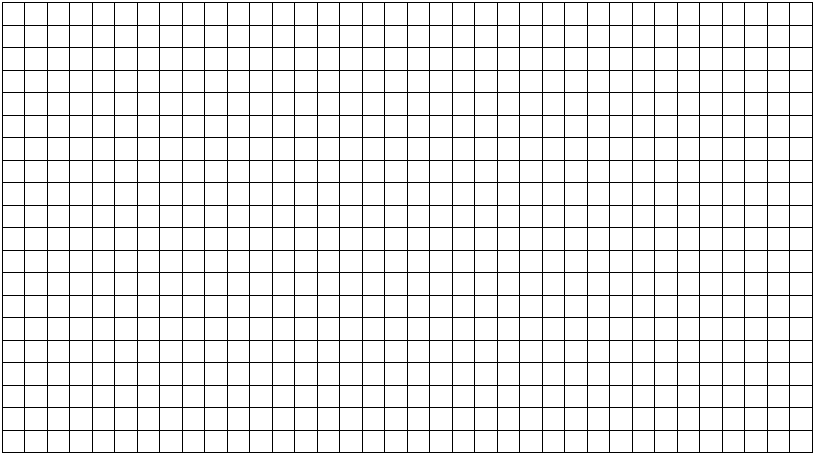
\includegraphics[width=\linewidth]{mesh_orthogonal.pdf}\\[-0.2em]
        \textbf{(a)} Orthogonal mesh
    \end{minipage}\hfill
    \begin{minipage}[t]{0.485\textwidth}
        \centering
        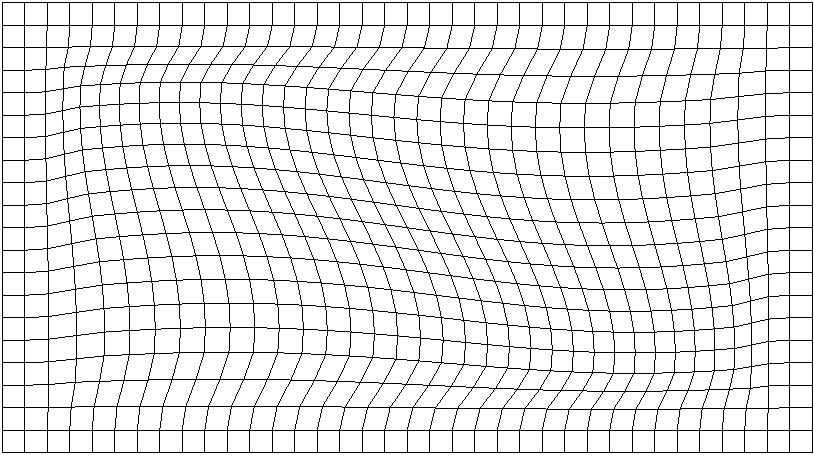
\includegraphics[width=\linewidth]{mesh_warpedInterior.pdf}\\[-0.2em]
        \textbf{(b)} Non-orthogonal interior mesh
    \end{minipage}
    \caption{Representative homogeneous-baseline meshes at
    $N_\lambda=32$.  The non-orthogonal interior mesh retains one orthogonal
    boundary-cell layer and introduces the deformation smoothly towards the
    interior.  \schematicAidDisclosure}
    \label{fig:homogeneousMeshes}
\end{figure}

\paperinput{homogeneous_convergence_table.tex}

\begin{figure}[htbp]
    \centering
    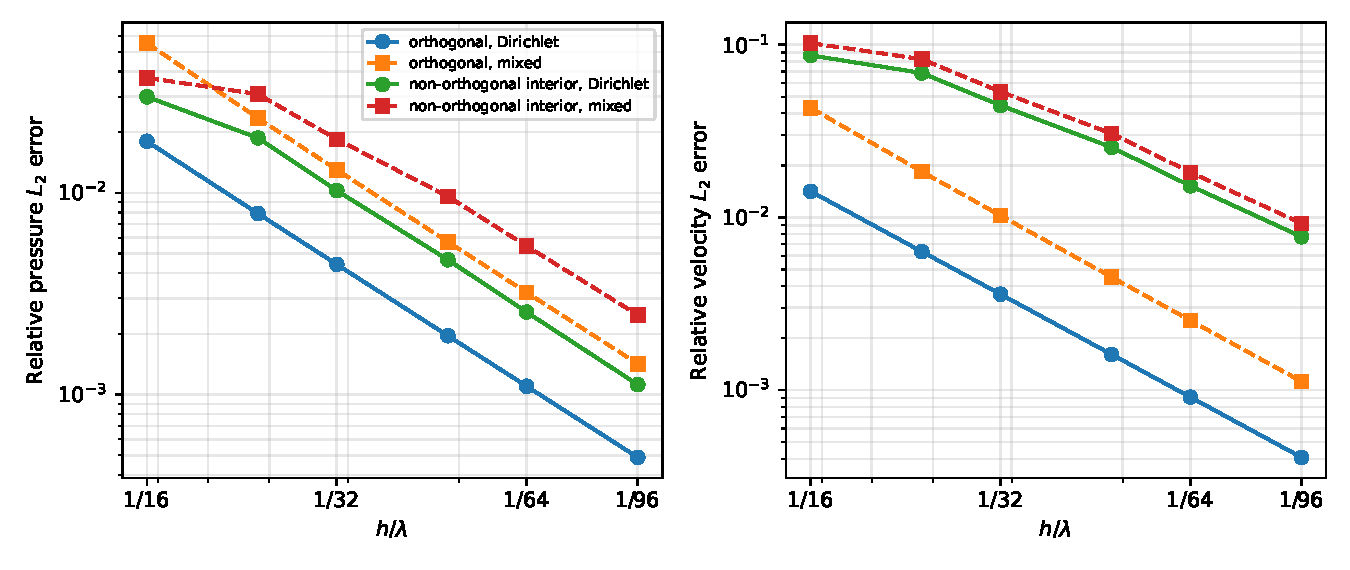
\includegraphics[width=0.95\textwidth]{figure05.pdf}
    \caption{Homogeneous plane-wave pressure and velocity convergence on
    orthogonal and non-orthogonal interior meshes.  The latter retain one orthogonal
    boundary-cell layer.  \plotAidDisclosure}
    \label{fig:homogeneousConvergence}
\end{figure}

The orthogonal results give $q_P=2.00$--$2.01$ on the finest interval and
approximately second-order velocity convergence for both boundary treatments.
On the non-orthogonal interior mesh family, the finest pressure orders are $2.04$ for the
Dirichlet case and $1.94$ for the mixed case.  The corresponding velocity
orders are $1.67$ and $1.68$, showing that gradient reconstruction remains more
sensitive to mesh deformation than the primary pressure solution.

\subsection{Layered gas--liquid interface with PML}
\label{sec:layeredInterface}
\label{sec:combinedInterfacePML}

After isolating the homogeneous operator, the next case tests the material
discontinuity and domain truncation in the same calculation.  The
heterogeneous material representation and the PML are assessed together
with a transducer-driven one-dimensional gas--liquid configuration.  A
prescribed normal velocity
$u_0=0.01\,\mathrm{m\,s^{-1}}$ at $x=0$ excites the gas at
$f=20\,\mathrm{kHz}$.  The gas--liquid interface is at
$L_1=0.09\,\mathrm{m}$, the liquid PML starts at $L_2=0.20\,\mathrm{m}$, and
the domain ends at $L=0.35\,\mathrm{m}$.  The gas properties are
$(\rho_1,c_1)=(1.2\,\mathrm{kg\,m^{-3}},343\,\mathrm{m\,s^{-1}})$ and the
liquid properties are
$(\rho_2,c_2)=(1000\,\mathrm{kg\,m^{-3}},1500\,\mathrm{m\,s^{-1}})$.  The PML uses
$\sigma_{\max}=5\times10^5\,\mathrm{s^{-1}}$ and polynomial order $p=3$.
The complete configuration is shown in \cref{fig:combinedLayeredSchematic}.

\begin{figure}[htbp]
    \centering
    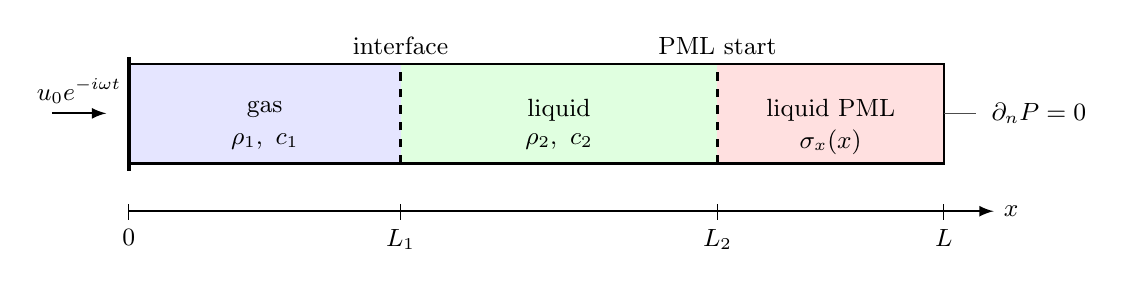
\begin{tikzpicture}[x=1.15cm,y=1.1cm,>=latex,font=\small]
        \def\xzero{0}
        \def\xone{3.0}
        \def\xtwo{6.5}
        \def\xthree{9.0}
        \def\h{1.15}

        \fill[blue!10] (\xzero,0) rectangle (\xone,\h);
        \fill[green!12] (\xone,0) rectangle (\xtwo,\h);
        \fill[red!12] (\xtwo,0) rectangle (\xthree,\h);
        \draw[thick] (\xzero,0) rectangle (\xthree,\h);
        \draw[thick,dashed] (\xone,0) -- (\xone,\h);
        \draw[thick,dashed] (\xtwo,0) -- (\xtwo,\h);

        \draw[very thick] (\xzero,-0.08) -- (\xzero,\h+0.08);
        \draw[->,thick] (-0.85,0.58) -- (-0.25,0.58)
            node[midway,above] {$u_0e^{-i\omega t}$};

        \node at (1.5,0.62) {gas};
        \node at (1.5,0.25) {$\rho_1,\ c_1$};
        \node at (4.75,0.62) {liquid};
        \node at (4.75,0.25) {$\rho_2,\ c_2$};
        \node at (7.75,0.62) {liquid PML};
        \node at (7.75,0.25) {$\sigma_x(x)$};

        \draw[->,thick] (\xzero,-0.55) -- (9.55,-0.55) node[right] {$x$};
        \foreach \x/\lab in
            {\xzero/$0$,\xone/$L_1$,\xtwo/$L_2$,\xthree/$L$}
        {
            \draw (\x,-0.47) -- (\x,-0.65);
            \node[below] at (\x,-0.65) {\lab};
        }
        \node[above] at (\xone,\h) {interface};
        \node[above] at (\xtwo,\h) {PML start};
        \draw[black!70] (\xthree,0.58) -- (9.35,0.58);
        \node[anchor=west] at (9.42,0.58) {$\partial_nP=0$};
    \end{tikzpicture}
    \caption{Configuration of the integrated one-dimensional layered-interface
    and directional-PML verification case.  \schematicAidDisclosure}
    \label{fig:combinedLayeredSchematic}
\end{figure}

For the continuous directional PML, the analytical pressure is
\begin{equation}
P(x)=
\begin{cases}
\rho_1c_1u_0
\dfrac{e^{ik_1x}+Re^{ik_1(2L_1-x)}}{1-Re^{i2k_1L_1}},
&0<x<L_1,\\[2ex]
\rho_1c_1u_0
\dfrac{1+R}{1-Re^{i2k_1L_1}}
e^{i[k_2(x-L_1)+k_1L_1]},
&L_1<x<L_2,\\[2ex]
e^{-\frac{\sigma_{\max}(L-L_2)}{(p+1)c_2}
\left(\frac{x-L_2}{L-L_2}\right)^{p+1}}
\rho_1c_1u_0
\dfrac{1+R}{1-Re^{i2k_1L_1}}
e^{i[k_2(x-L_1)+k_1L_1]},
&L_2<x<L,
\end{cases}
\label{eq:combinedLayeredPMLAnalytical}
\end{equation}
where $k_j=\omega/c_j$ and
$R=(\rho_2c_2-\rho_1c_1)/(\rho_2c_2+\rho_1c_1)$.

\begin{figure}[htbp]
    \centering
    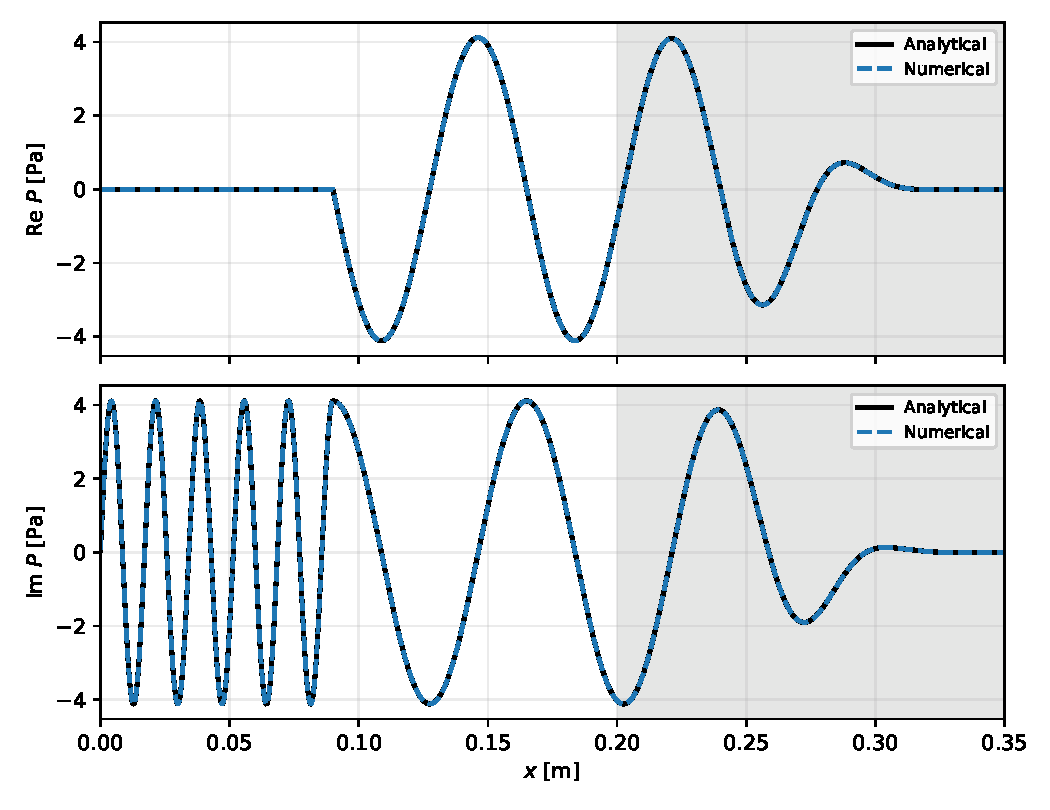
\includegraphics[width=0.78\textwidth]{figure07.pdf}
    \caption{Integrated layered-interface--PML case: numerical real and
    imaginary pressure components compared with the analytical solution.  The
    shaded region denotes the PML.  \plotAidDisclosureRevision}
    \label{fig:combinedLayeredPressure}
\end{figure}

\begin{figure}[htbp]
    \centering
    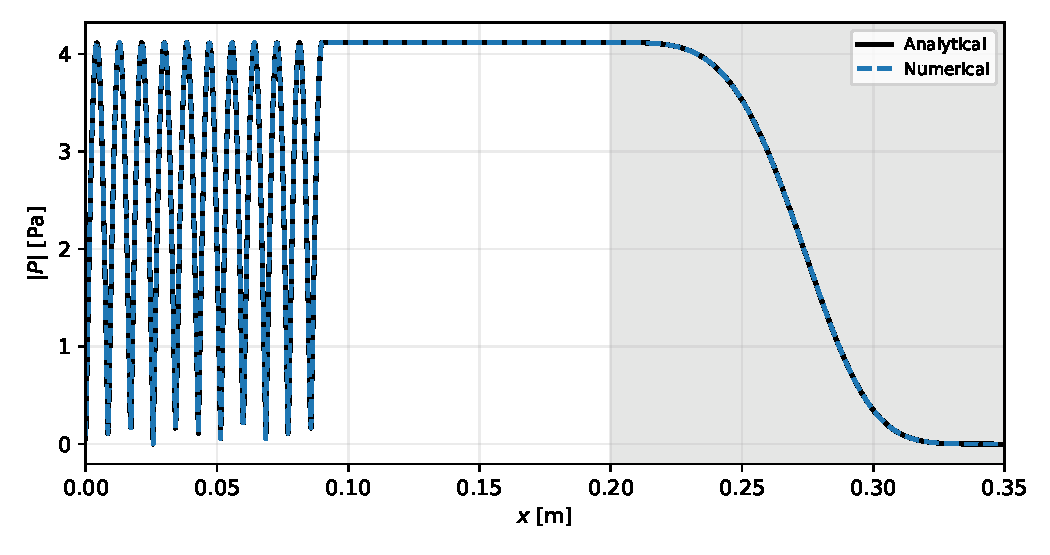
\includegraphics[width=0.78\textwidth]{figure08.pdf}
    \caption{Integrated layered-interface--PML case: numerical and analytical
    pressure amplitude, including attenuation through the directional PML.  \plotAidDisclosureRevision}
    \label{fig:combinedLayeredAmplitude}
\end{figure}

On the $N_x=8000$ mesh, the complex-pressure error from
\cref{eq:errorMeasures}, evaluated at the cell centres of the complete
interval $0\leq x\leq L$ including the PML, is $E_P=1.163\times10^{-3}$.
Here, $L_1$ lies inside a
cell rather than on a mesh face, so the interface position enters through the
cell values of \cref{eq:materialAverages}.  A single comparison thus covers
the reflected and transmitted fields and their attenuation in the PML.
\Cref{fig:combinedLayeredPressure} shows the real and imaginary components,
and \cref{fig:combinedLayeredAmplitude} the amplitude with its constant
transmitted value and its decay through the PML.

As an additional reverse-incidence check, the two materials are interchanged so
that the wave travels from water into air, while the geometry, excitation, and
PML parameters remain unchanged.  The pressure reflection coefficient is then
$R=-0.999451$, corresponding to an almost complete phase-reversed reflection
and a much smaller transmitted pressure in air.  The numerical and analytical
complex pressures remain in close agreement over the complete domain in
\cref{fig:combinedLayeredWaterAir}, with $E_P=4.430\times10^{-3}$.

\begin{figure}[H]
    \centering
    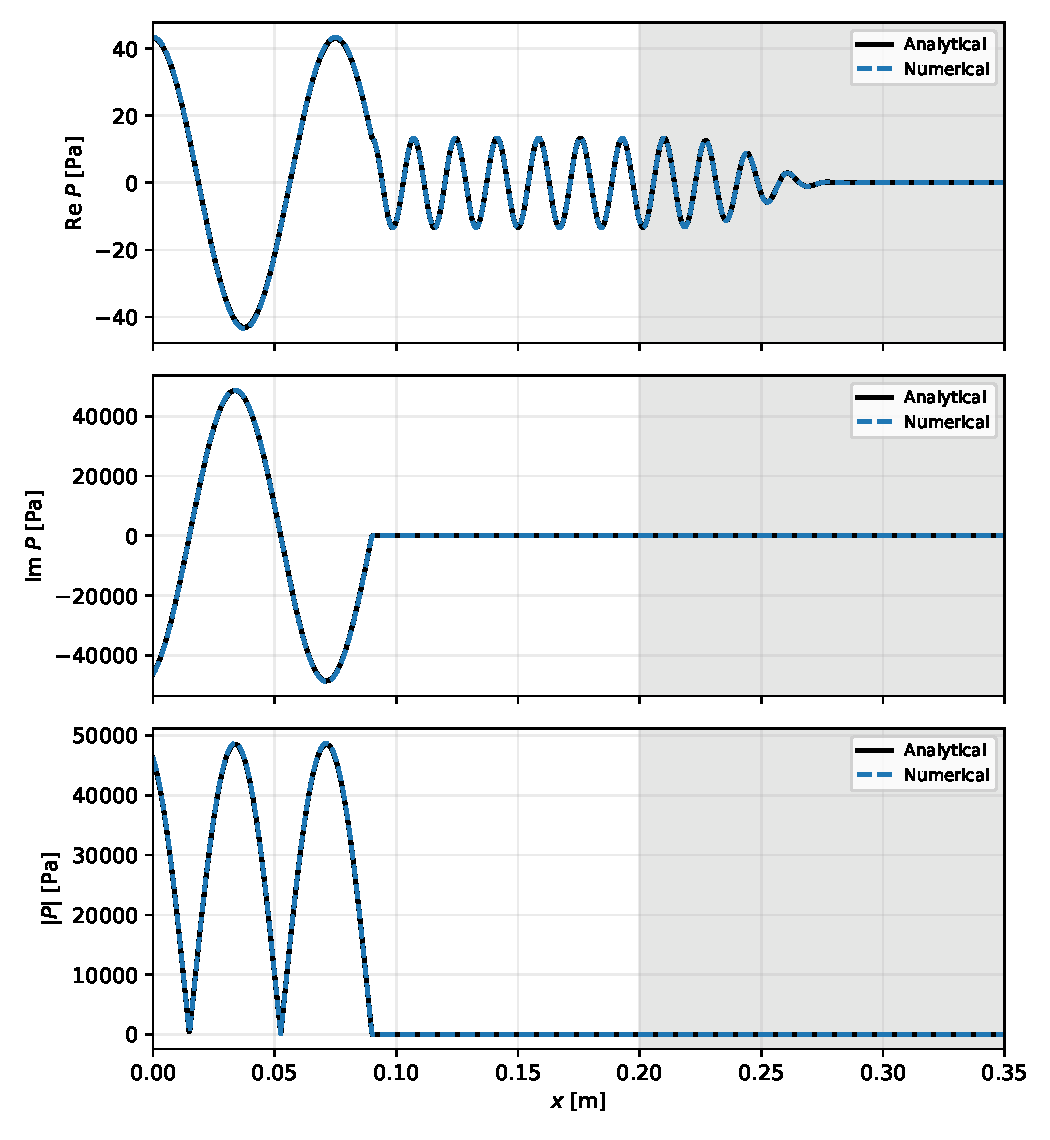
\includegraphics[width=0.70\textwidth]{figure09.pdf}
    \caption{Reverse layered-interface--PML check: numerical and analytical
    pressure for propagation from water into air.  The upper panels show the
    real and imaginary components, and the lower panel shows the amplitude.
    The pressure approaches a node at the interface; the shaded region denotes
    the air-side PML.  \plotAidDisclosureRevision}
    \label{fig:combinedLayeredWaterAir}
\end{figure}

\FloatBarrier
\subsubsection{PML damping and mesh sensitivity}
\label{sec:pmlSensitivity}

The PML parameters are studied with the same layered configuration as in \cref{fig:combinedLayeredSchematic} and the
same whole-domain complex-pressure error.  First, $N_x=8000$, the PML thickness,
and $p=3$ are held fixed while $\sigma_{\max}$ is varied.  The results in
\cref{tab:pmlSigmaSensitivity,fig:pmlSigmaSensitivity} show that weak damping
does not sufficiently attenuate the wave before the outer boundary.  Increasing
$\sigma_{\max}$ from $10^4$ to $5\times10^5\,\mathrm{s^{-1}}$ reduces $E_P$
from $5.189\times10^{-1}$ to $1.163\times10^{-3}$.

\paperinput{pml_sigma_sensitivity_table.tex}

\begin{figure}[htbp]
    \centering
    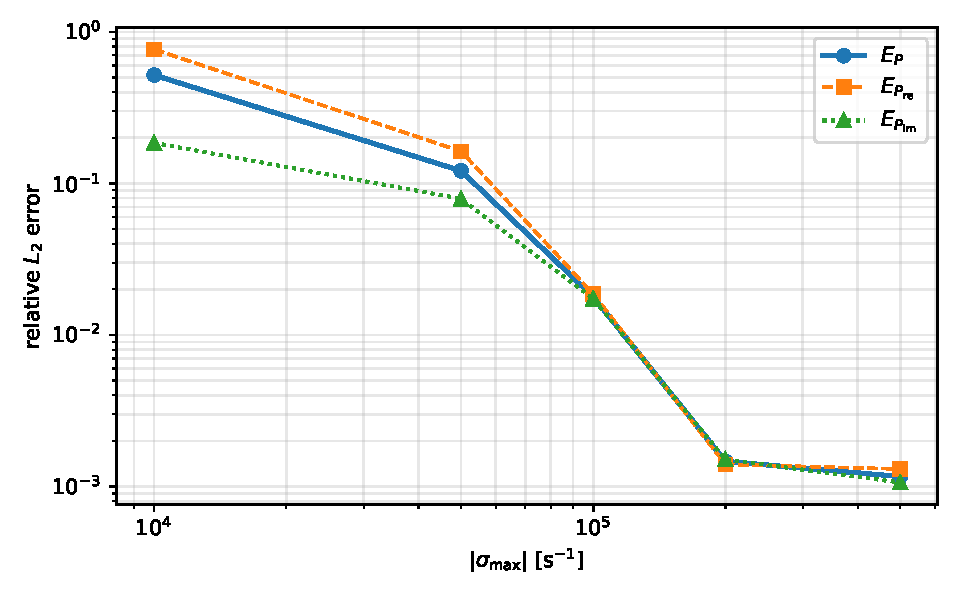
\includegraphics[width=0.75\textwidth]{figure10.pdf}
    \caption{Whole-domain complex-pressure and component errors for the layered
    gas--liquid--PML case as functions of maximum PML damping.  \plotAidDisclosure}
    \label{fig:pmlSigmaSensitivity}
\end{figure}

For the resolution study, $\sigma_{\max}=5\times10^5\,\mathrm{s^{-1}}$ is
fixed and the mesh is refined while keeping the material interface and PML
start aligned with mesh faces.  \Cref{tab:pmlMeshSensitivity,fig:pmlMeshSensitivity}
show second-order convergence of $E_P$, from $1.960\times10^{-2}$ at
$N_x=560$ to $7.844\times10^{-5}$ at $N_x=8960$, with observed orders between
$1.98$ and $2.00$.  With the interface inside a cell, the error at
$N_x=8000$ is $1.163\times10^{-3}$, about fifteen times that on the aligned
mesh with $N_x=8960$.

\paperinput{pml_mesh_sensitivity_table.tex}

\begin{figure}[htbp]
    \centering
    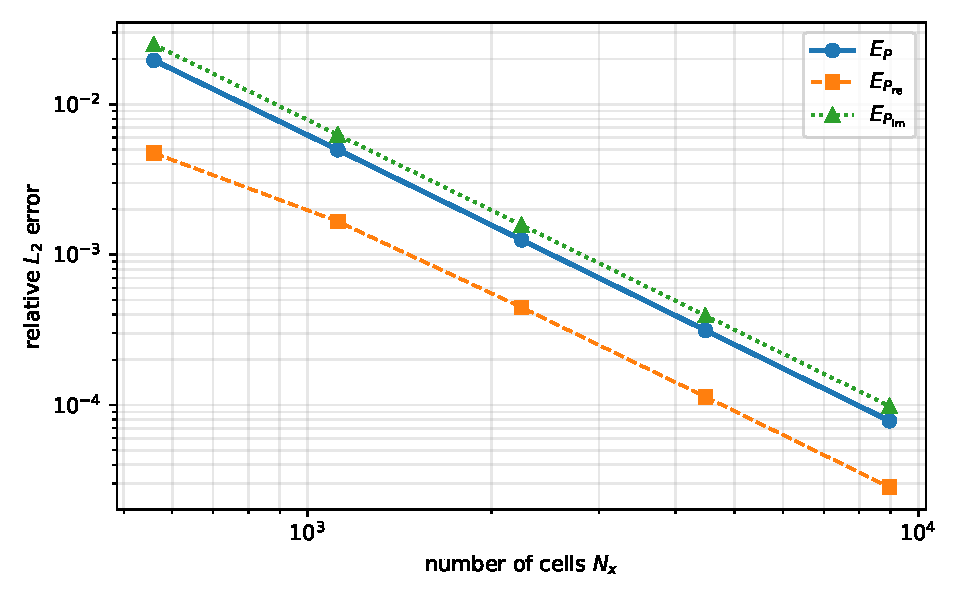
\includegraphics[width=0.75\textwidth]{figure11.pdf}
    \caption{Whole-domain complex-pressure and component errors under aligned
    mesh refinement for the layered gas--liquid--PML case.  \plotAidDisclosure}
    \label{fig:pmlMeshSensitivity}
\end{figure}

\FloatBarrier
\subsection{Controlled comparison of face-area definitions}
\label{sec:geometricComparison}

To isolate the effect of \cref{eq:averagedFaceFraction}, we compare the
original donor-based face-area selection with geometric averaging while
retaining the flux in \cref{eq:retainedInterfaceFlux}; everything else,
including the mesh and the initial interface, is identical.  For all layered
cases of \cref{sec:layeredInterface,sec:pmlSensitivity}, solved on one, four
and eight ranks, the two selections give identical pressure fields, and
parallel fields differ from serial ones by at most $1.95\times10^{-12}$.

A curved-interface comparison uses a penetrable liquid sphere of radius
$a=1\,\mathrm{mm}$ centred in the cube $[-2a,2a]^3$.  The liquid and gas
properties are those of \cref{sec:layeredInterface}.  An incident plane wave
$P_{\mathrm{inc}}=1\,\mathrm{Pa}\,e^{ik_gx}$ has $k_ga=1$.
The independent reference matches regular interior spherical-Bessel and
outgoing exterior spherical-Hankel expansions through continuity of
pressure and of $\rho^{-1}\partial_nP$ at $r=a$ \cite{anderson1950sound},
retaining angular orders $0$--$24$.  Its total complex pressure supplies
Dirichlet data on the cube boundary, so no PML is used in this comparison.  The cell-centred
numerical pressure is compared with this reference using cell-volume
weights.  Decomposition dependence is measured after reconstructing the
parallel field in the original cell ordering as
\begin{equation}
 D_8=\frac{\lVert P_h^{(8)}-P_h^{(1)}\rVert_V}
                {\lVert P_h^{(1)}\rVert_V}.
 \label{eq:parallelPressureDifference}
\end{equation}

\paperinput{geometric_comparison_table.tex}

\Cref{tab:geometricComparison} reports all four tested resolutions.
On the finest mesh, geometric averaging changes $E_P$ from $2.9746\%$
to $2.9753\%$, while reducing $D_8$ from $2.64\times10^{-6}$ to roundoff,
below $10^{-14}$.  The true relative assembled residual is below $10^{-10}$ in these
sphere and layered runs.  These results motivate the
selection through reproducibility with essentially unchanged pressure accuracy.

\FloatBarrier
\subsection{Penetrable sphere with PML truncation}
\label{sec:spherePML}

The sphere in \cref{sec:geometricComparison} is bounded by exact pressure
data, so it does not involve the PML.  The present case combines a curved
transmitting interface, the axisymmetric discretization and the PML in one
calculation.  A sphere of radius $a=1\,\mathrm{mm}$ is centred on the axis of
a one-degree wedge and is represented only by its volume fraction.  An axial
point source at $y=2.5a$ radiates into the surrounding medium; it is realized
as an excluded cylinder of radius $a/4$ and height $a/2$ on the axis whose
faces carry the exact pressure.  The physical region $r\leq4a$,
$-4a\leq y\leq6a$ has uniform cells of size $h=a/N$, $N=8$--$64$, and $ka=1$
in the surrounding medium.  The finest mesh has $163\,328$ cells in the
physical region and $489\,472$ cells including the PML.  The geometry is
shown in \cref{fig:spherePMLSetup}.  The reference pressure is the point-source field plus the field
scattered by the fluid sphere.  The point-source field is expanded in Legendre
polynomials with the addition theorem \cite[(10.60.1), (10.60.2)]{NIST:DLMF},
and the scattering coefficients follow from continuity of pressure and of
$\rho^{-1}\partial_nP$ at $r=a$ as for an incident plane wave
\cite{anderson1950sound}; the expansion retains angular orders $0$--$60$.

\begin{figure}[htbp]
    \centering
    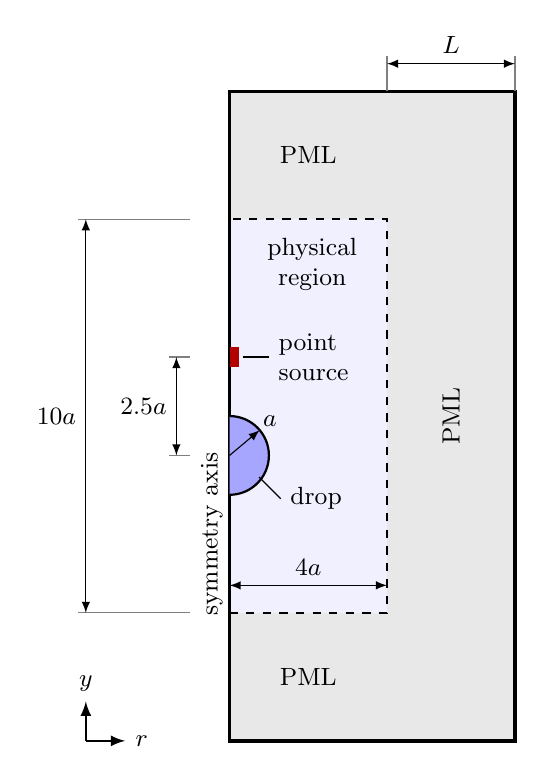
\begin{tikzpicture}[x=0.5cm,y=0.5cm,>=latex,font=\small]
        % Meridional plane in units of a: physical region r <= 4a,
        % -4a <= y <= 6a; PML of thickness L = 3.25a on three sides.
        \def\rp{4}\def\ylo{-4}\def\yhi{6}\def\pml{3.25}
        \pgfmathsetmacro{\ro}{\rp+\pml}
        \pgfmathsetmacro{\yo}{\ylo-\pml}
        \pgfmathsetmacro{\yt}{\yhi+\pml}

        \fill[gray!18] (0,\yo) rectangle (\ro,\yt);
        \fill[blue!6] (0,\ylo) rectangle (\rp,\yhi);
        \draw[very thick] (0,\yo) rectangle (\ro,\yt);
        \draw[dashed,thick] (0,\ylo) -- (\rp,\ylo) -- (\rp,\yhi) -- (0,\yhi);

        % Drop and excluded source cylinder on the axis.
        \fill[blue!35] (0,1) arc[start angle=90,end angle=-90,radius=1] -- cycle;
        \draw[thick] (0,1) arc[start angle=90,end angle=-90,radius=1];
        \fill[red!70!black] (0,2.25) rectangle (0.25,2.75);
        \draw[->] (0,0) -- (40:1) node[above right,inner sep=1pt] {$a$};

        \draw (0.35,2.5) -- (1.0,2.5) node[right,align=left] {point\\source};
        \draw (0.75,-0.55) -- (1.3,-1.1) node[right] {drop};
        \node[align=center] at (2.1,4.85) {physical\\region};
        \node[rotate=90] at ({\rp+0.5*\pml},1) {PML};
        \node at (2,{\yhi+0.5*\pml}) {PML};
        \node at (2,{\ylo-0.5*\pml}) {PML};

        % Dimensions.
        \draw[gray] (-1.0,0) -- (-1.55,0);
        \draw[gray] (-1.0,2.5) -- (-1.55,2.5);
        \draw[<->] (-1.35,0) -- (-1.35,2.5) node[midway,left] {$2.5a$};
        \draw[gray] (-1.0,\ylo) -- (-3.85,\ylo);
        \draw[gray] (-1.0,\yhi) -- (-3.85,\yhi);
        \draw[<->] (-3.65,\ylo) -- (-3.65,\yhi) node[midway,left] {$10a$};
        \draw[<->] (0,-3.3) -- (\rp,-3.3) node[midway,above] {$4a$};
        \draw[gray] (\rp,\yt) -- (\rp,{\yt+0.9});
        \draw[gray] (\ro,\yt) -- (\ro,{\yt+0.9});
        \draw[<->] (\rp,{\yt+0.7}) -- (\ro,{\yt+0.7}) node[midway,above] {$L$};
        \node[rotate=90] at (-0.45,-2.0) {symmetry axis};

        % Coordinates.
        \draw[->,thick] (-3.65,{\yo}) -- (-2.65,{\yo}) node[right] {$r$};
        \draw[->,thick] (-3.65,{\yo}) -- (-3.65,{\yo+1}) node[above] {$y$};
    \end{tikzpicture}
    \caption{Penetrable sphere with PML truncation: meridional plane of the
    one-degree wedge, to scale for $L=3.25a$.  The point source is an excluded
    cylinder on the axis whose faces carry the exact pressure.  The outer
    boundary of the PML has $\partial_nP=0$.  With exact boundary data, the
    mesh ends at the dashed boundary of the physical region.
    \schematicAidDisclosureRevision}
    \label{fig:spherePMLSetup}
\end{figure}

Two material pairs are considered.  A water drop
$(1000\,\mathrm{kg\,m^{-3}},1500\,\mathrm{m\,s^{-1}})$ in air
$(1.2\,\mathrm{kg\,m^{-3}},343\,\mathrm{m\,s^{-1}})$ represents the
high-contrast water--air regime of \cref{sec:application}.  Its analytical
exterior field differs from that of
a rigid sphere by only $1.9\times10^{-4}$, measured with
\cref{eq:errorMeasures} over the exterior part of the physical region.  An oil
drop $(920\,\mathrm{kg\,m^{-3}},1450\,\mathrm{m\,s^{-1}})$ in water has a low
impedance contrast; its exterior field differs from the rigid-sphere field by
$0.14$, so transmission substantially affects this exterior field.  The
domain is truncated either by the exact pressure on the outer boundary of the
physical region or by a PML of thickness $L=3.25a=0.52\lambda$ with
$\sigma_{\max}/\omega=12.6$, $p=3$ and the azimuthal damping of
\cref{eq:wedgeAzimuthalStretch}.  The damping ratio equals that of the
levitator in \cref{sec:application}.

\paperinput{sphere_pml_table.tex}

The PML errors in \cref{tab:spherePML} are slightly below those obtained
with exact boundary data and decrease at the same rate.  For the oil drop the observed order is $2.0$ on all intervals.  For the
water drop it decreases from $1.7$ to $1.05$; nearly the same orders occur
with exact boundary data, which is consistent with an error associated with
the curved material interface rather than PML truncation.  Without the azimuthal damping of
\cref{eq:wedgeAzimuthalStretch}, the error stops decreasing at about $3\%$ for
both drops.  Solutions on
eight ranks differ from the serial solutions by at most $3.4\times10^{-14}$
for $N=16$ and $32$, and the true relative assembled residual is below
$2\times10^{-13}$ in all runs.

\FloatBarrier
\subsection{Baffled-piston radiation}
\label{sec:piston}

A rigid circular piston of radius $a$ oscillates with normal velocity
amplitude $u_0$ in an infinite rigid baffle.  This classical radiation problem
has an exact solution in the whole radiated field, so propagation, radiation
into the PML and the axisymmetric discretization are tested together against
the same reference.  The numerical domain is truncated by a rectangular PML.
The case uses $f=10\,\mathrm{kHz}$, $a=0.1\,\mathrm{m}$,
$(\rho_0,c)=(1.2\,\mathrm{kg\,m^{-3}},343\,\mathrm{m\,s^{-1}})$, a
$2^\circ$ axisymmetric wedge, and a rectangular meridional domain
$0\leq x,y\leq0.28\,\mathrm{m}$.  The PML starts at $x=0.20\,\mathrm{m}$ and
$y=0.20\,\mathrm{m}$, giving a thickness of $0.08\,\mathrm{m}$ along the outer
radial and upper boundaries.  To preserve the geometry during refinement, a
radial block boundary is placed exactly at $x=a$ and directly separates the
driven piston patch from the rigid baffle.  The geometry is shown in
\cref{fig:pistonConfiguration}.

\begin{figure}[H]
    \centering
    \resizebox{0.52\textwidth}{!}{%
    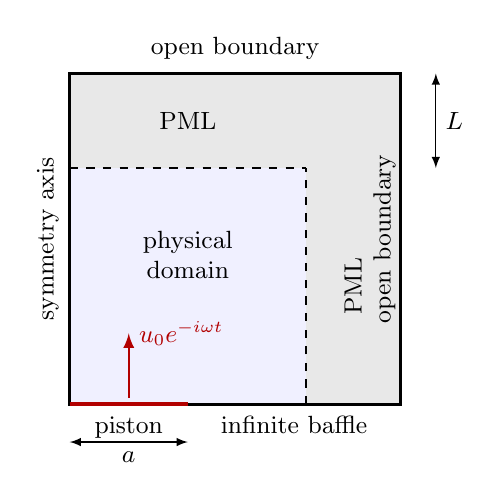
\begin{tikzpicture}[x=1cm,y=1cm,>=latex,font=\small]
        \def\inner{3.0}
        \def\outer{4.2}
        \def\piston{1.5}

        \fill[blue!6] (0,0) rectangle (\inner,\inner);
        \fill[gray!18] (\inner,0) rectangle (\outer,\outer);
        \fill[gray!18] (0,\inner) rectangle (\inner,\outer);
        \draw[very thick] (0,0) rectangle (\outer,\outer);
        \draw[dashed,thick] (\inner,0) -- (\inner,\inner);
        \draw[dashed,thick] (0,\inner) -- (\inner,\inner);

        \draw[red!70!black,line width=1.5pt] (0,0) -- (\piston,0);
        \draw[very thick] (\piston,0) -- (\outer,0);
        \draw[<->] (0,-0.48) -- (\piston,-0.48)
            node[midway,below] {$a$};
        \draw[->,red!70!black,thick] (0.75,0.08) -- (0.75,0.90)
            node[right] {$u_0e^{-i\omega t}$};

        \draw[<->] (4.65,\inner) -- (4.65,\outer)
            node[midway,right] {$L$};

        \node[rotate=90] at (-0.28,2.1) {symmetry axis};
        \node[align=center] at (1.5,1.9) {physical\\domain};
        \node[rotate=90] at (3.60,1.50) {PML};
        \node at (1.50,3.60) {PML};
        \node[below] at (0.75,-0.03) {piston};
        \node[below] at (2.85,-0.03) {infinite baffle};
        \node[above] at (2.1,{\outer+0.06}) {open boundary};
        \node[rotate=90,above] at ({\outer+0.06},2.1) {open boundary};
    \end{tikzpicture}
    }
    \caption{Axisymmetric baffled-piston configuration.  The rectangular PML
    occupies the outer radial and upper strips and their corner.  The
    numerical pressure is compared with the exact field in the physical
    domain.  \schematicAidDisclosure}
    \label{fig:pistonConfiguration}
\end{figure}

For the $e^{-i\omega t}$ convention of \cref{as:timeHarmonic}, the radiated
pressure is given by the Rayleigh integral \cite{morse1986theoretical}
\begin{equation}
    P(\x)
    =
    -\frac{i\omega\rho_0u_0}{2\pi}
    \int_{S_p}\frac{e^{ikR}}{R}\,dS_{\mathbf y},
    \qquad
    R=|\x-\mathbf y|,
    \label{eq:pistonRayleigh}
\end{equation}
where $S_p$ is the piston surface.  Let $r$ and $z$ denote the distances of
$\x$ from the symmetry axis and from the baffle.  In polar coordinates
$(\varrho,\varphi)$ centred at the projection of $\x$ onto the baffle plane,
$R\,dR=\varrho\,d\varrho$, so the radial integration in
\cref{eq:pistonRayleigh} is exact.  For $r\leq a$, the projection lies on the
piston and
\begin{equation}
    P(r,z)
    =
    \rho_0cu_0
    \left[
    e^{ikz}
    -\frac{1}{2\pi}\int_0^{2\pi}e^{ikR_e(\varphi)}\,d\varphi
    \right],
    \label{eq:pistonEdgeInside}
\end{equation}
with $R_e=(z^2+\varrho_e^2)^{1/2}$ and
$\varrho_e=-r\cos\varphi+(a^2-r^2\sin^2\varphi)^{1/2}$ the distance from the
projection to the rim.  The pressure is thus a plane wave minus an edge wave
emitted by the piston rim.  For $r>a$, the rays with
$|\varphi|<\varphi_0=\arcsin(a/r)$ cross the piston between $\varrho_1$ and
$\varrho_2$, and
\begin{equation}
    P(r,z)
    =
    -\frac{\rho_0cu_0}{2\pi}
    \int_{-\varphi_0}^{\varphi_0}
    \left[e^{ikR_2(\varphi)}-e^{ikR_1(\varphi)}\right]d\varphi,
    \label{eq:pistonEdgeOutside}
\end{equation}
with $R_j=(z^2+\varrho_j^2)^{1/2}$ and
$\varrho_{1,2}=r\cos\varphi\mp(a^2-r^2\sin^2\varphi)^{1/2}$.  On the axis, $R_e=\sqrt{z^2+a^2}$ is constant and \cref{eq:pistonEdgeInside}
reduces to the closed form
\begin{equation}
    |P|(0,z)
    =
    2\rho_0cu_0
    \left|
    \sin\left[
    \frac{k}{2}\left(\sqrt{z^2+a^2}-z\right)
    \right]
    \right|.
    \label{eq:pistonNearField}
\end{equation}
Unlike \cref{eq:pistonRayleigh}, whose integrand becomes nearly singular
next to the piston, the one-dimensional integrals in
\cref{eq:pistonEdgeInside,eq:pistonEdgeOutside} remain smooth up to the
baffle.  They are evaluated by Gauss--Legendre quadrature; the result agrees
with \cref{eq:pistonNearField} on the axis and with a direct quadrature of
\cref{eq:pistonRayleigh} away from the baffle to within
$2\times10^{-13}\rho_0cu_0$.

The numerical pressure is compared with the reference at the cell centres,
without interpolation or extrapolation.  The field error $E_P^{\Omega}$ is
$E_P$ in \cref{eq:complexPressureErrors} over all cells of the physical domain
$0\leq x,y\leq0.20\,\mathrm{m}$ with $w_i=V_i$.  In the wedge, $V_i$ is
proportional to the distance from the axis, so $E_P^{\Omega}$ is the relative
$L^2$ error over the corresponding three-dimensional region; it includes the
cells next to the PML and therefore also measures reflections from the layer.
The axis errors $E_P^{\mathrm{axis}}$ and
\begin{equation}
    E_\infty^{\mathrm{axis}}
    =\frac{\max_i|P_h(\x_i)-P_{\mathrm{ex}}(\x_i)|}
          {\max_i|P_{\mathrm{ex}}(\x_i)|}
    \label{eq:pistonAxisErrors}
\end{equation}
use the cell row adjacent to the symmetry axis with $w_i=1$.

\paperinput{piston_convergence_table.tex}

\begin{figure}[H]
    \centering
    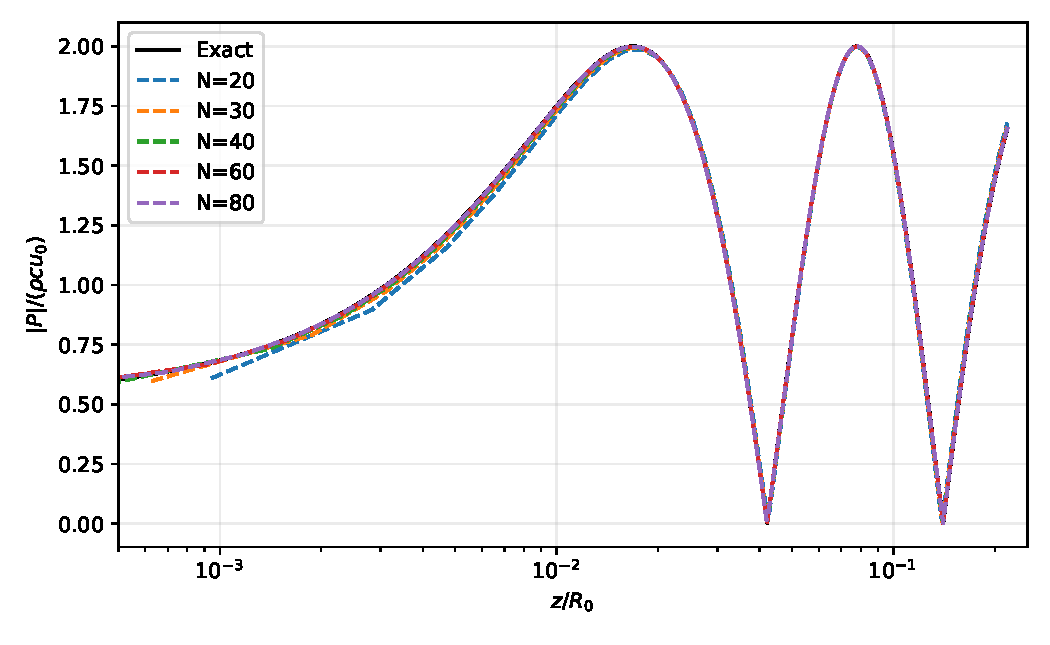
\includegraphics[width=0.85\textwidth]{piston_axis_cpc.pdf}
    \caption{Baffled-piston radiation: pressure amplitude in the cell row
    adjacent to the symmetry axis on five meshes, compared with
    \cref{eq:pistonNearField}; $R_0=ka^2/2$ is the Rayleigh distance.
    \plotAidDisclosureRevision}
    \label{fig:pistonNearAmpMethod}
\end{figure}

\begin{figure}[H]
    \centering
    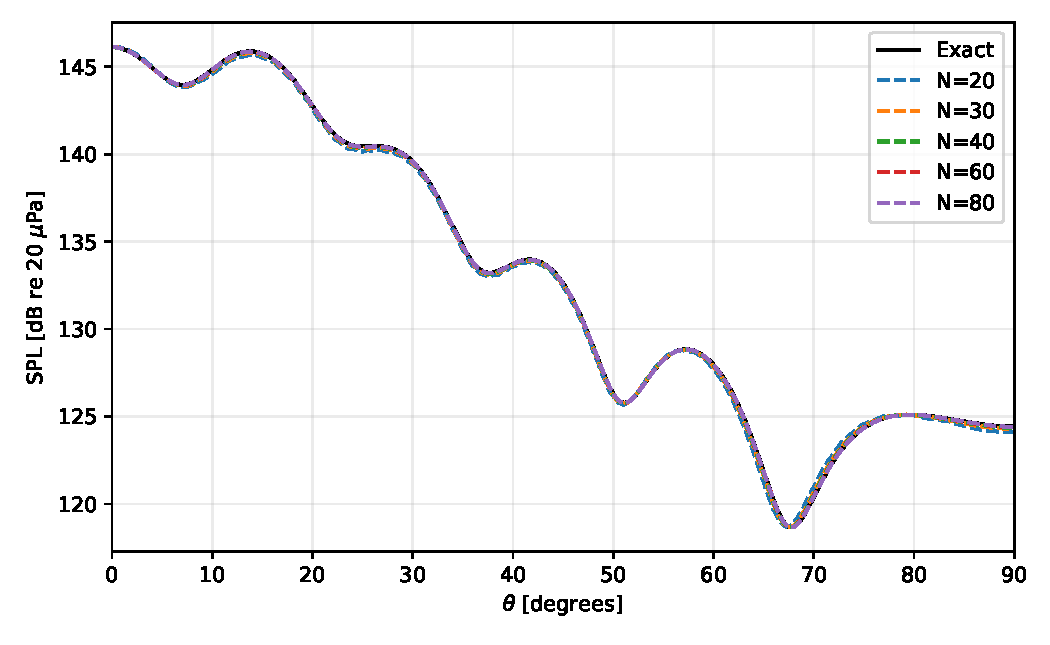
\includegraphics[width=0.85\textwidth]{piston_arc_cpc.pdf}
    \caption{Baffled-piston radiation: sound pressure level on the arc of
    radius $0.18\,\mathrm{m}$ around the piston centre, as a function of the
    angle $\theta$ from the symmetry axis, on five meshes compared with the
    exact field, with
    $\mathrm{SPL}=20\log_{10}\bigl(|P|/(\sqrt2\,p_{\mathrm{ref}})\bigr)$ and
    $p_{\mathrm{ref}}=20\,\mu\mathrm{Pa}$.  The numerical values are
    interpolated to the arc for plotting only.  \plotAidDisclosureRevision}
    \label{fig:pistonArcLevel}
\end{figure}

\begin{figure}[H]
    \centering
    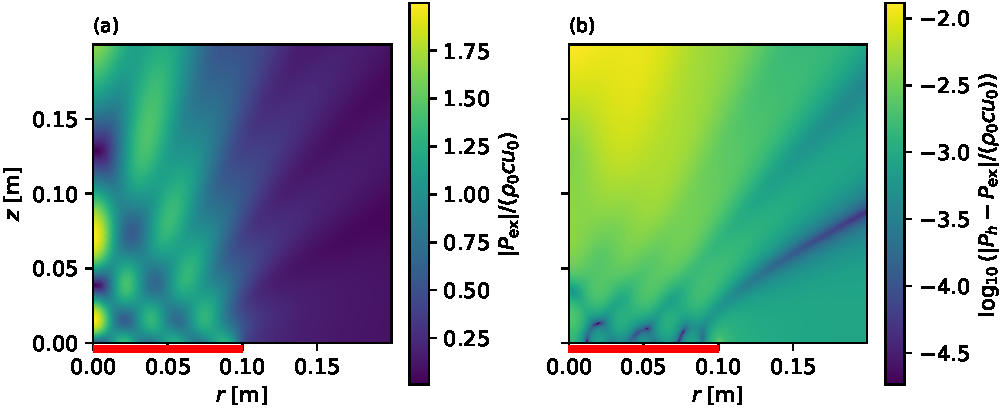
\includegraphics[width=\textwidth]{piston_error_cpc.pdf}
    \caption{Baffled-piston radiation in the physical domain on the finest
    mesh (80 cells per wavelength): (a) exact pressure amplitude; (b)
    pointwise error of the complex pressure.  The red line marks the piston;
    the PML starts at the upper and right edges of the plotted region.
    \plotAidDisclosureRevision}
    \label{fig:pistonErrorMap}
\end{figure}

\Cref{tab:pistonConvergence} shows second-order convergence of the complex
pressure.  The field error $E_P^{\Omega}$ decreases from
$8.63\times10^{-2}$ at 20 cells per wavelength to $5.26\times10^{-3}$ at 80
cells per wavelength, with observed orders between $1.99$ and $2.05$; the axis
errors converge at the same rate.  Because $E_P^{\Omega}$ extends to the PML
interface, the convergence also shows no error floor from PML reflections down
to the finest mesh.  \Cref{fig:pistonNearAmpMethod,fig:pistonArcLevel} show
that the computed amplitude follows the exact solution through the on-axis
interference minima and over the side lobes of the angular pattern; on the
coarsest mesh, the largest visible deviation occurs close to the piston
surface.

\Cref{fig:pistonErrorMap} shows where the error arises on the finest mesh.
It grows with the propagation distance along the main beam, from about
$2\times10^{-3}\rho_0cu_0$ near the piston to about $10^{-2}\rho_0cu_0$ at
$z=0.2\,\mathrm{m}$, and its amplitude part is an order of magnitude smaller
than the complex error, with root-mean-square values of $2.8\times10^{-4}$ and
$2.7\times10^{-3}$ relative to $\rho_0cu_0$.  The error is therefore mainly
the phase error of numerical dispersion.  It increases at the same rate up to
the PML interface, without a local rise there.  Next to the baffle, the
largest errors occur within a few cells of the piston rim, where the
prescribed velocity is discontinuous.

\FloatBarrier
\subsection{Rigid-sphere radiation force in a standing wave}
\label{sec:gorkovVerification}

The radiation-pressure quantity in \cref{eq:acousticRadiationPressure} is
verified by resolving a sound-hard sphere in a one-dimensional standing wave.
This homogeneous-gas case tests radiation-stress postprocessing separately
from the transmitting liquid interface and the PML.
With a rigid reflector at $y=0$, the incident complex pressure and velocity are
\begin{equation}
    P_{\mathrm{inc}}(y)=P_a\cos(ky),
    \qquad
    \V_{\mathrm{inc}}(y)=
    i\frac{P_a}{\rho_0c}\sin(ky)\,\mathbf e_y,
    \label{eq:gorkovStandingWave}
\end{equation}
which is consistent with the $e^{-i\omega t}$ convention in
\cref{as:timeHarmonic}.  For a spherical particle in the Rayleigh regime,
$ka\ll1$, with volume $V_p=4\pi a^3/3$, the Gorkov potential is
\cite{gorkov1962potential}
\begin{equation}
    U_G=V_p\left[
        \frac{f_1|P_{\mathrm{inc}}|^2}{4\rho_0c^2}
        -\frac{3f_2\rho_0|\V_{\mathrm{inc}}|^2}{8}
    \right].
    \label{eq:gorkovPotential}
\end{equation}
Consequently, the axial force is
\begin{equation}
    F_{G,y}=-\frac{\mathrm dU_G}{\mathrm dy}
    =4\pi a^3kE_{\mathrm{ac}}\Phi\sin(2ky),
    \qquad
    E_{\mathrm{ac}}=\frac{P_a^2}{4\rho_0c^2},
    \qquad
    \Phi=\frac{f_1}{3}+\frac{f_2}{2}.
    \label{eq:gorkovForce}
\end{equation}
The sound-hard, acoustically rigid limit has $f_1=f_2=1$ and hence
$\Phi=5/6$.

The numerical force is obtained from the time-averaged radiation-stress
traction on the resolved sphere,
\begin{equation}
    \mathbf F_h=
    \int_{\partial\Omega_p}
    \left[
        p_{\mathrm{rad}}\mathbf I
        +\frac{\rho_0}{2}
        \left(
            \V_{\mathrm{re}}\V_{\mathrm{re}}
            +\V_{\mathrm{im}}\V_{\mathrm{im}}
        \right)
    \right]\cdot\mathbf n_f\,\mathrm dA,
    \label{eq:resolvedRadiationForce}
\end{equation}
where $\mathbf n_f$ points out of the fluid and into the sphere.  The
momentum-flux term vanishes on an exactly sound-hard wall.

The cylindrical cavity has height $H=7.64\,\mathrm{mm}$ and equal transducer
and reflector radii of $10\,\mathrm{mm}$.  The reflector and cylindrical side
wall are rigid.  At the transducer, the analytical value
$P(H)=P_a\cos(kH)$ is imposed with $P_a=1\,\mathrm{Pa}$,
$f=25.25\,\mathrm{kHz}$, $\rho_0=1.2\,\mathrm{kg\,m^{-3}}$, and
$c=343\,\mathrm{m\,s^{-1}}$.  Thus, only the excitation is prescribed; the
total pressure and scattered field around the sphere are computed.  No PML is
active in this closed-cavity reference problem.  The computational domain and
boundary conditions are summarized in \cref{fig:gorkovDomainSchematic}.

\begin{figure}[htbp]
    \centering
    \begin{minipage}[t]{0.58\textwidth}
    \centering
    \resizebox{\linewidth}{!}{%
    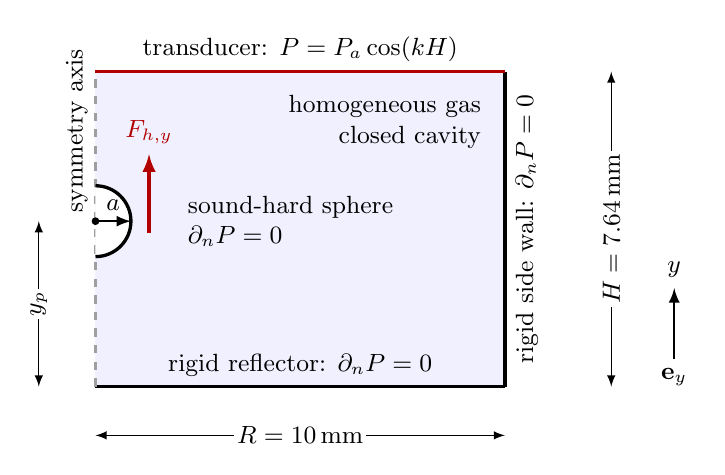
\begin{tikzpicture}[x=1cm,y=1cm,>=latex,font=\small]
        \def\domainR{5.2}
        \def\domainH{4.0}
        \def\particleY{2.1}
        \def\particleR{0.45}

        % Meridional half-domain of the axisymmetric cavity.
        \fill[blue!6] (0,0) rectangle (\domainR,\domainH);
        \draw[very thick] (0,0) -- (\domainR,0);
        \draw[very thick] (\domainR,0) -- (\domainR,\domainH);
        \draw[red!70!black,very thick] (0,\domainH) --
            (\domainR,\domainH);
        \draw[gray!75,dashed,thick] (0,0) -- (0,\domainH);

        % Resolved sphere: a semicircle in the meridional half-domain.
        \fill[white]
            (0,{\particleY+\particleR})
            arc[start angle=90,end angle=-90,radius=\particleR] -- cycle;
        \draw[black,very thick]
            (0,{\particleY+\particleR})
            arc[start angle=90,end angle=-90,radius=\particleR];
        \fill (0,\particleY) circle (1.4pt);
        \draw[->,thick] (0,\particleY) -- (\particleR,\particleY)
            node[midway,above] {$a$};
        \draw[->,red!70!black,very thick]
            (0.68,{\particleY-0.15}) -- (0.68,{\particleY+0.85})
            node[above] {$F_{h,y}$};

        % Geometry dimensions.
        \draw[<->] (-0.72,0) -- (-0.72,\particleY)
            node[midway,fill=white,inner sep=1pt,rotate=90] {$y_p$};
        \draw[<->] (6.55,0) -- (6.55,\domainH)
            node[midway,fill=white,inner sep=1pt,rotate=90]
            {$H=7.64\,\mathrm{mm}$};
        \draw[<->] (0,-0.62) -- (\domainR,-0.62)
            node[midway,fill=white,inner sep=1pt]
            {$R=10\,\mathrm{mm}$};

        % Boundary-condition and domain labels.
        \node[above] at ({0.5*\domainR},\domainH)
            {transducer: $P=P_a\cos(kH)$};
        \node[above] at ({0.5*\domainR},0)
            {rigid reflector: $\partial_nP=0$};
        \node[rotate=90,fill=white,inner sep=1pt] at
            (5.48,{0.5*\domainH})
            {rigid side wall: $\partial_nP=0$};
        \node[rotate=90,fill=white,inner sep=1pt] at (-0.24,3.25)
            {symmetry axis};
        \node[align=left,anchor=west] at (1.05,\particleY)
            {sound-hard sphere\\$\partial_nP=0$};
        \node[anchor=north east,align=right] at
            ({\domainR-0.18},{\domainH-0.18})
            {homogeneous gas\\closed cavity};

        \draw[->,thick] (7.35,0.35) -- (7.35,1.25)
            node[above] {$y$};
        \node at (7.35,0.12) {$\mathbf e_y$};
    \end{tikzpicture}
    }\\[-0.2em]
    \textbf{(a)} Domain and boundary conditions
    \end{minipage}\hfill
    \begin{minipage}[t]{0.38\textwidth}
    \centering
    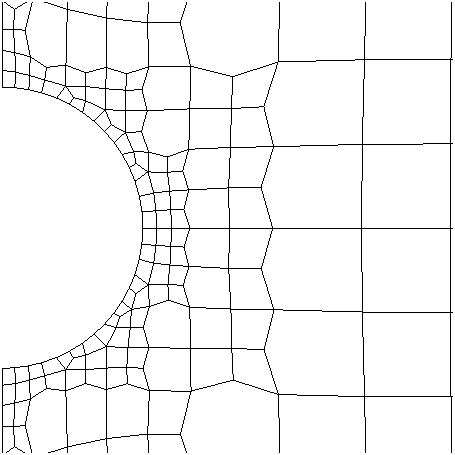
\includegraphics[width=\linewidth]{mesh_gorkov.pdf}\\[-0.2em]
    \textbf{(b)} Local mesh
    \end{minipage}
    \caption{Rigid-sphere Gorkov case: (a) closed cavity and boundary
    conditions, with the sphere enlarged; (b) illustrative local mesh at
    $h_s/a=0.2$.  Quantitative levels are listed in
    \cref{tab:gorkovMeshConvergence}.  The mesh is a $1^\circ$ axisymmetric
    wedge; no PML is active.  OpenAI Codex (model \texttt{gpt-6-astra}) assisted with the schematic and mesh-rendering code; the mesh is regenerated from the case setup.}
    \label{fig:gorkovDomainSchematic}
\end{figure}

The axisymmetric unstructured meshes contain approximately $2.2\times10^4$
cells, with $35^\circ$--$42^\circ$ maximum and less than $2.1^\circ$ average
non-orthogonality.  The prescribed local cell size adjacent to the sphere is
denoted by $h_s$, and $h_s/a$ is the dimensionless near-sphere resolution.
\Cref{tab:gorkovMeshConvergence} and
\cref{fig:gorkovMeshConvergence} show the near-sphere refinement study at
$a=60\,\mu\mathrm{m}$ and $y=4.0003\,\mathrm{mm}$.  Refining from
$h_s/a=1/8$ to $1/16$ changes the force by $2.665\%$; the change from $1/16$ to
$1/32$ is $0.199\%$.  The medium and fine results differ from the Gorkov value
by $0.105\%$ and $0.095\%$, respectively.  The medium level is therefore used
for the parameter sweeps.

\paperinput{gorkov_mesh_convergence_table.tex}

\begin{figure}[htbp]
    \centering
    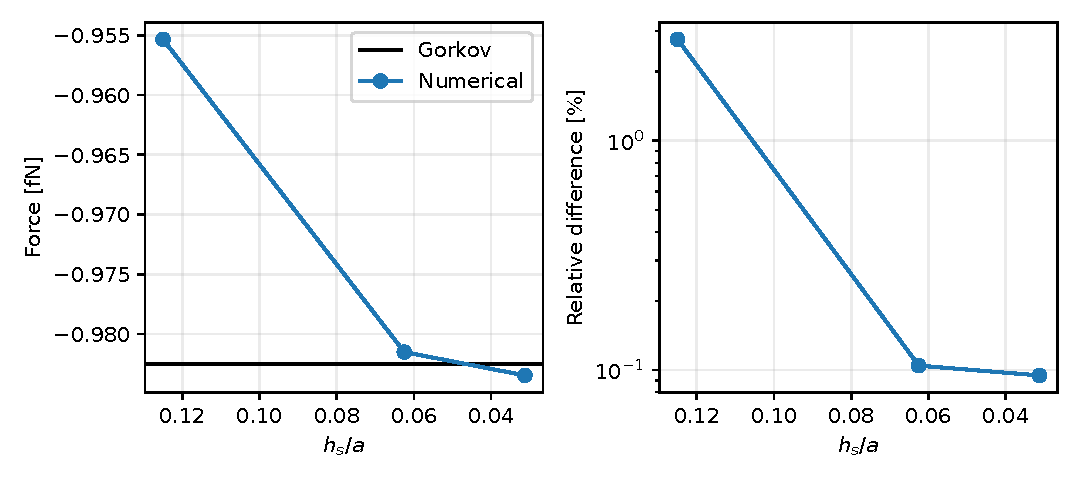
\includegraphics[width=0.92\textwidth]{figure17.pdf}
    \caption{Rigid-sphere force sensitivity to the near-sphere cell size and
    surface segmentation.  \plotAidDisclosure}
    \label{fig:gorkovMeshConvergence}
\end{figure}

The radius sweep covers $30\leq a\leq150\,\mu\mathrm{m}$, corresponding to
$0.0139\leq ka\leq0.0694$.  The numerical force follows the expected
$a^3$ scaling, and the maximum difference from \cref{eq:gorkovForce} is
$1.485\%$, as shown in \cref{fig:gorkovRadiusSweep}.  This range remains in the
Rayleigh regime required by the point-particle reference.

\begin{figure}[htbp]
    \centering
    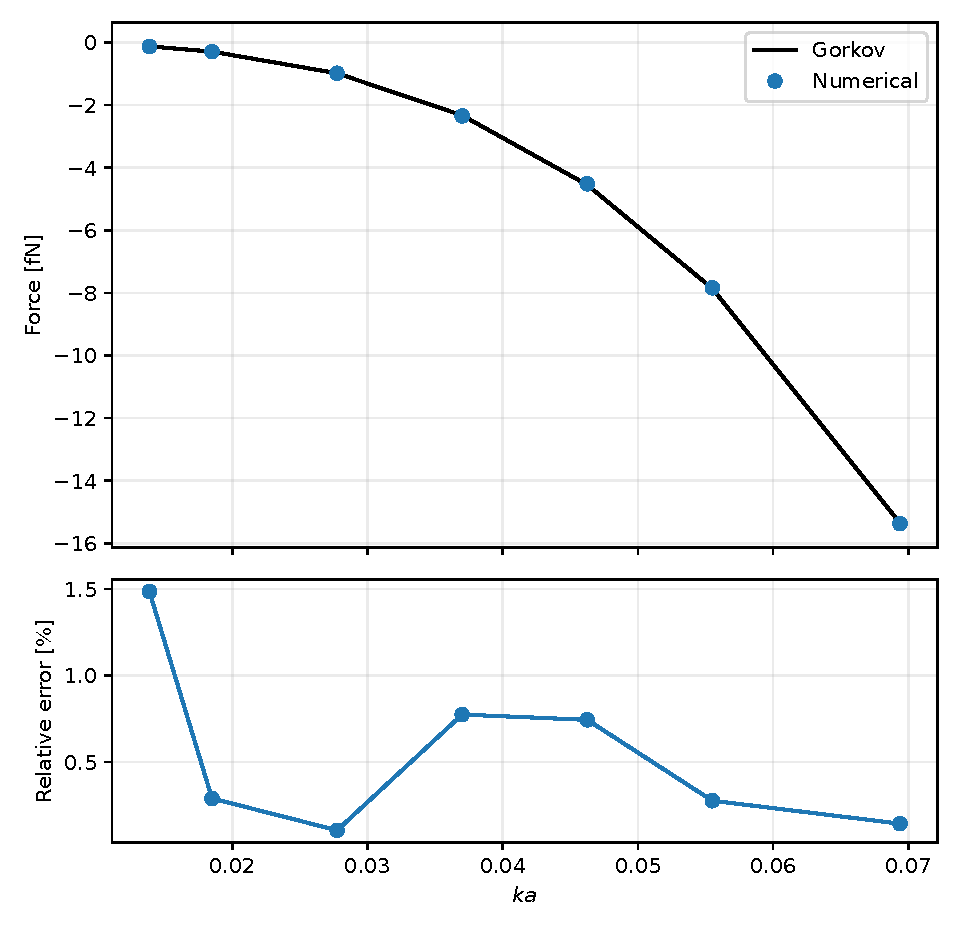
\includegraphics[width=0.82\textwidth]{figure18.pdf}
    \caption{Resolved rigid-sphere force and Gorkov prediction over the
    Rayleigh size-parameter range.  \plotAidDisclosure}
    \label{fig:gorkovRadiusSweep}
\end{figure}

Finally, a $60\,\mu\mathrm{m}$ sphere is moved through the standing wave.  The
resolved force reproduces both force lobes, their signs, and the two analytical
zero crossings in the cavity, as shown in \cref{fig:gorkovPositionSweep}.  The
root-mean-square force difference is $1.288\%$ of the peak Gorkov force.  The
maximum peak-normalized difference is $3.415\%$ at the first analytical zero;
there the numerical residual is $0.0633\,\mathrm{fN}$.

\begin{figure}[htbp]
    \centering
    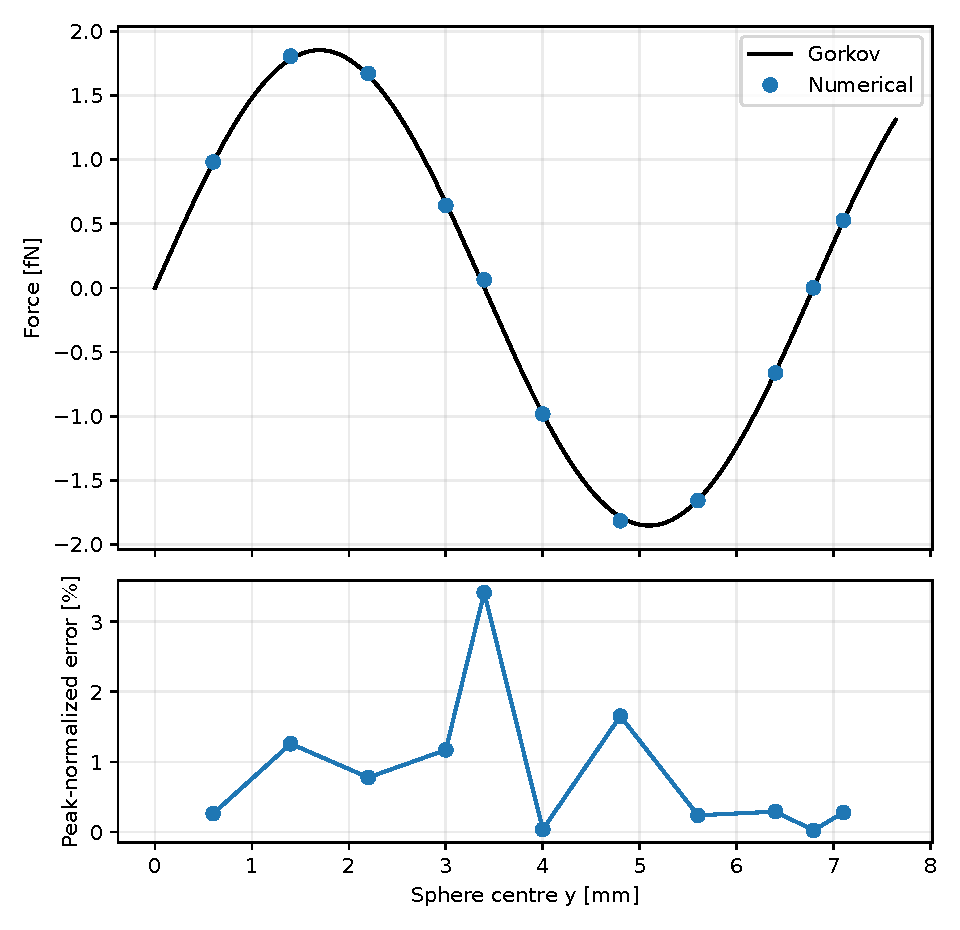
\includegraphics[width=0.88\textwidth]{figure19.pdf}
    \caption{Axial radiation force on a $60\,\mu\mathrm{m}$ rigid sphere as a
    function of its vertical position.  The error is normalized by the peak
    analytical force.  \plotAidDisclosure}
    \label{fig:gorkovPositionSweep}
\end{figure}

\section{Application to a levitator with prescribed liquid drops}
\label{sec:application}

The preceding studies assess separate numerical requirements.  A
transducer--reflector levitator combines a curved liquid inclusion, an
unstructured mesh, directional PML truncation and an observable device force.
We use the height-sweep example of the companion software preprint
\cite{Xu2026AcousticHelmholtzFoam}, based on the configuration of Andrade and
Marzo \cite{andrade2019numerical}, to demonstrate this combined calculation.
The measured quantity is the mean force on the reflector.

\begin{figure}[htbp]
    \centering
    \begin{minipage}[t]{0.62\textwidth}
    \centering
    \resizebox{\linewidth}{!}{%
    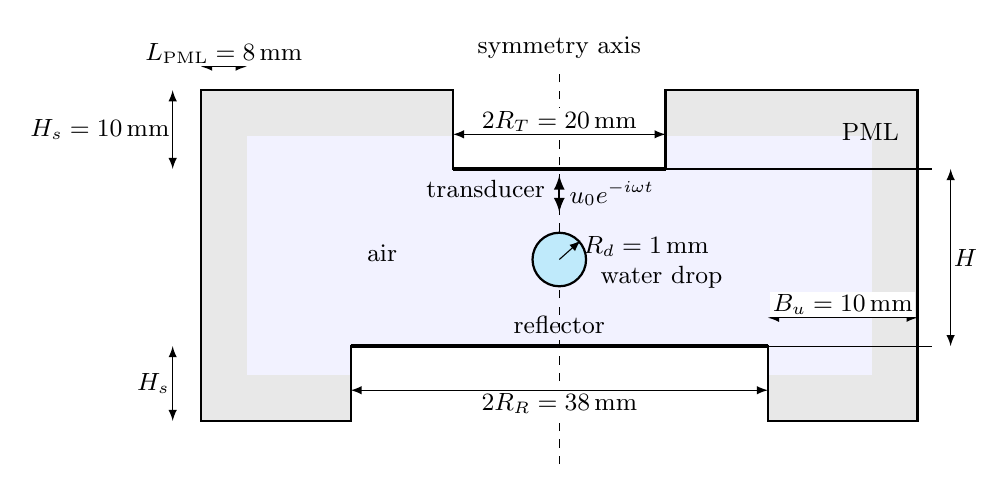
\begin{tikzpicture}[x=1cm,y=1cm,>=latex,font=\small]
        \def\xouter{4.55}
        \def\xref{2.65}
        \def\xtr{1.35}
        \def\pmlt{0.58}
        \def\ybot{-0.95}
        \def\yref{0.00}
        \def\ydrop{1.10}
        \def\yface{2.25}
        \def\ytop{3.25}
        \def\dropR{0.34}

        \fill[blue!5]
            (-\xouter,\ybot) -- (-\xouter,\ytop) -- (-\xtr,\ytop)
            -- (-\xtr,\yface) -- (\xtr,\yface) -- (\xtr,\ytop)
            -- (\xouter,\ytop) -- (\xouter,\ybot) -- (\xref,\ybot)
            -- (\xref,\yref) -- (-\xref,\yref) -- (-\xref,\ybot) -- cycle;

        \fill[gray!18] (-\xouter,\ybot) rectangle ({-\xouter+\pmlt},\ytop);
        \fill[gray!18] ({\xouter-\pmlt},\ybot) rectangle (\xouter,\ytop);
        \fill[gray!18] (-\xouter,{\ytop-\pmlt}) rectangle (-\xtr,\ytop);
        \fill[gray!18] (\xtr,{\ytop-\pmlt}) rectangle (\xouter,\ytop);
        \fill[gray!18] (-\xouter,\ybot) rectangle (-\xref,{\ybot+\pmlt});
        \fill[gray!18] (\xref,\ybot) rectangle (\xouter,{\ybot+\pmlt});

        \draw[thick]
            (-\xouter,\ybot) -- (-\xouter,\ytop) -- (-\xtr,\ytop)
            -- (-\xtr,\yface) -- (\xtr,\yface) -- (\xtr,\ytop)
            -- (\xouter,\ytop) -- (\xouter,\ybot) -- (\xref,\ybot)
            -- (\xref,\yref) -- (-\xref,\yref) -- (-\xref,\ybot) -- cycle;
        \draw[dashed] (0,{\ybot-0.55}) -- (0,{\ytop+0.28})
            node[above] {symmetry axis};
        \draw[line width=1.45pt] (-\xtr,\yface) -- (\xtr,\yface);
        \draw[<->,thick] (0,{\yface-0.08}) -- (0,{\yface-0.55})
            node[midway,right] {$u_0 e^{-i\omega t}$};
        \node[below left] at (-0.06,{\yface-0.02}) {transducer};
        \draw[line width=1.45pt] (-\xref,\yref) -- (\xref,\yref);
        \node[above] at (0,{\yref+0.03}) {reflector};
        \fill[cyan!25] (0,\ydrop) circle (\dropR);
        \draw[thick] (0,\ydrop) circle (\dropR);
        \draw[->] (0,\ydrop) -- (0.27,1.34)
            node[pos=0.68,right] {$R_d=1\,\mathrm{mm}$};
        \node[right] at (0.40,0.87) {water drop};
        \node at (-2.25,1.18) {air};
        \node at (3.95,2.72) {PML};

        \draw[<->] ({\xouter+0.42},\yref) -- ({\xouter+0.42},\yface)
            node[midway,right,fill=white,inner sep=1pt] {$H$};
        \draw (\xtr,\yface) -- ({\xouter+0.18},\yface);
        \draw (\xref,\yref) -- ({\xouter+0.18},\yref);
        \draw[<->] (-\xtr,{\yface+0.44}) -- (\xtr,{\yface+0.44})
            node[midway,above,fill=white,inner sep=1pt] {$2R_T=20\,\mathrm{mm}$};
        \draw[<->] (-\xref,{\yref-0.56}) -- (\xref,{\yref-0.56})
            node[midway,below,fill=white,inner sep=1pt] {$2R_R=38\,\mathrm{mm}$};
        \draw[<->] (\xref,0.36) -- (\xouter,0.36)
            node[midway,above,fill=white,inner sep=1pt] {$B_u=10\,\mathrm{mm}$};
        \draw[<->] (-\xouter,{\ytop+0.30}) -- ({-\xouter+\pmlt},{\ytop+0.30})
            node[midway,above,fill=white,inner sep=1pt] {$L_{\mathrm{PML}}=8\,\mathrm{mm}$};
        \draw[<->] ({-\xouter-0.36},\yface) -- ({-\xouter-0.36},\ytop)
            node[midway,left,fill=white,inner sep=1pt] {$H_s=10\,\mathrm{mm}$};
        \draw[<->] ({-\xouter-0.36},\ybot) -- ({-\xouter-0.36},\yref)
            node[midway,left,fill=white,inner sep=1pt] {$H_s$};
    \end{tikzpicture}
    }
    \end{minipage}
    \hfill
    \begin{minipage}[t]{0.31\textwidth}
    \centering
    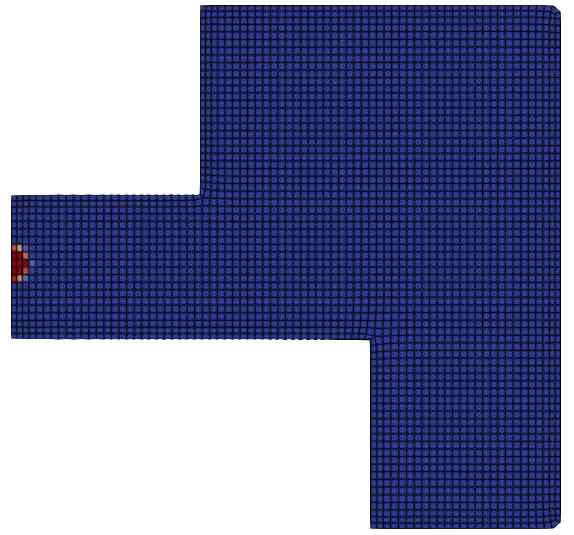
\includegraphics[width=\linewidth]{../helmholtz_software/mesh_levitator.png}
    \end{minipage}
    \caption{Schematic meridional view of the single-axis levitator used in the
    application example.  The transducer--reflector spacing $H$ is swept, the
    reference drop is placed at mid-height, and the rectangular PML regions
    are indicated by the shaded bands.  The right panel shows the
    corresponding one-degree wedge mesh generated with cfMesh, with cells
    where $\alpha=1$ marked in red.  The geometry and mesh illustration are
    reused from the companion software preprint
    \cite{Xu2026AcousticHelmholtzFoam}.}
    \label{fig:cpcLevitatorGeometry}
\end{figure}

\Cref{fig:cpcLevitatorGeometry} shows the axisymmetric arrangement, with
transducer and reflector diameters of $20$ and $38\,\mathrm{mm}$,
respectively.  A one-degree wedge represents the acoustic domain.  The drop is
centred at mid-height and described by a liquid volume fraction, with density
and compressibility assigned through \cref{eq:materialAverages}.  A spherical
drop of radius $1\,\mathrm{mm}$ defines the reference volume.  Oblate
spheroids with equatorial-to-polar aspect ratios $a/b=1$, $2$ and $3$ retain
this volume.  Each shape remains fixed during its acoustic solve; an empty
levitator supplies the comparison without an inclusion. 

The frequency is $25.25\,\mathrm{kHz}$ and the transducer normal-velocity
amplitude is $1\,\mathrm{m\,s^{-1}}$.  The material properties are
$\rho_g=1.2\,\mathrm{kg\,m^{-3}}$, $c_g=343\,\mathrm{m\,s^{-1}}$,
$\rho_l=998.3\,\mathrm{kg\,m^{-3}}$ and
$c_l=1480\,\mathrm{m\,s^{-1}}$.  The reflector is sound-hard, while the
liquid is an acoustically transmitting medium.  Cartesian PML regions have
thickness $8\,\mathrm{mm}$, polynomial order $3$, and maximum damping
magnitude $2\times10^6\,\mathrm{s^{-1}}$ in the radial and axial directions.  For each configuration the spacing
$H$ takes 100 uniformly distributed values from $0.46\lambda_g$ to
$0.64\lambda_g$, where $\lambda_g=c_g/f$.

At the sound-hard reflector, the normal acoustic velocity and hence the normal
momentum-flux contribution vanish.  The force is evaluated from
\cref{eq:acousticRadiationPressure} in the homogeneous gas adjacent to the
reflector.  With $\Gamma_r$ denoting the reflector patch and $\mathbf n$ its
mean normal, the full axisymmetric force is
\begin{equation}
    F_n=\frac{360^\circ}{\theta_{\mathrm{wedge}}}
    \mathbf n\cdot\sum_{f\in\Gamma_r}
    p_{\mathrm{rad},f}\Sf,
    \qquad \theta_{\mathrm{wedge}}=1^\circ.
    \label{eq:cpcReflectorForce}
\end{equation}


\begin{figure}[htbp]
    \centering
    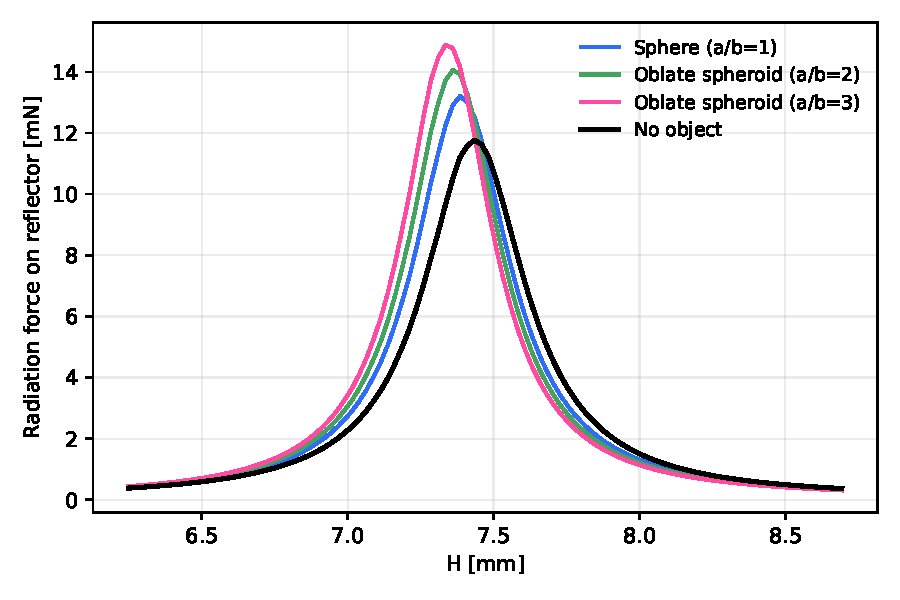
\includegraphics[width=0.92\textwidth]{../helmholtz_software/levitator_height_sweep.pdf}
    \caption{Mean force on the reflector during the levitator height sweep,
    for an empty levitator and constant-volume drops with prescribed aspect
    ratios.  Each curve contains 100 height samples.  The curves are
    reproduced from the companion software preprint
    \cite{Xu2026AcousticHelmholtzFoam}.}
    \label{fig:cpcLevitatorHeightSweep}
\end{figure}

In \cref{fig:cpcLevitatorHeightSweep}, inserting the drop shifts the
reflector-force response relative to the empty levitator.  Increasing the
aspect ratio shifts the response further towards smaller spacings and
increases the peak force in the plotted configurations.  Thus, prescribing the
same incident standing wave independently of the liquid geometry would omit
the observed change in device response.  The example demonstrates why the
liquid representation, device boundaries and open-domain treatment must be
used together when computing this response.


\FloatBarrier

\section{Discussion}
\label{sec:discussion}

The analytical reference fields in \cref{sec:spherePML} indicate how the
effect of transmission depends on the material pair in the tested
point-source configuration at $ka=1$.  For a water drop in air, the exterior
field differs from that of a rigid sphere by $1.9\times10^{-4}$; for an oil
drop in water, the difference is $0.14$.  The first comparison supports a
sound-hard approximation for the exterior field in this benchmark, consistent
with the modelling choice of Andrade and Marzo \cite{andrade2019numerical}.
The second shows a substantial transmission effect.  The present formulation
represents both material pairs and the interior field with the same
volume-fraction description, boundary conditions and mesh.  The levitator
height sweep demonstrates the response to prescribed drop shapes; the
contribution of transmission to its reflector force has not been isolated by
a matched sound-hard device calculation.

The same test shows where the accuracy of the volume-fraction representation
is limited.  With either truncation, the oil drop converges at second order
and the water drop at about first order on the finest meshes.  Since
geometry, meshes and truncation are identical in both cases, this difference
is consistent with sensitivity of the one-field cell and face closure
to material contrast at a curved interface.  Both density and sound speed
change between the two material pairs, so their separate effects are not
resolved by this comparison.  The layered case also shows sensitivity to
interface placement: it converges at second order when the interface coincides
with mesh faces, whereas an interface inside a cell increases the error
approximately fifteenfold.  The homogeneous and piston cases, which contain
no material interface, converge at second order.

On axisymmetric wedge meshes, Cartesian PML coefficients reproduce the
stretch of a radial layer only together with the azimuthal damping of
\cref{eq:wedgeAzimuthalStretch}.  Without this term, the error in
\cref{sec:spherePML} stagnates at approximately $3\%$ under mesh refinement.
Since the derivation in \cref{sec:wedgePML} does not rely on the
finite-volume discretization, the term is required by any axisymmetric
discretization that reuses Cartesian PML coefficients.

The formulation assumes a fixed interface during each solve and neglects
first-order capillary--acoustic coupling, and each PML must contain a
homogeneous continuation of the exterior medium.  Viscous and thermal
losses and acoustic streaming are not modelled, and the default sparse direct
factorization limits the size of three-dimensional calculations through its
memory requirements.

\section{Conclusions}
\label{sec:conclusions}

This work has developed a frequency-domain acoustic formulation for
heterogeneous gas--liquid media on unstructured finite-volume meshes, in which
geometrically reconstructed volume-of-fluid interfaces define the material
coefficients and perfectly matched layers truncate the open domain.  A VOF
representation of the two-phase interface, a cell-centred finite-volume
Helmholtz discretization and PML truncation are thereby combined in a single
acoustic calculation.  Because the liquid geometry enters only through the
volume fraction and the shared face coefficients derived from it, different
interface configurations are evaluated on a fixed mesh.  In contrast to
finite-element models with interface-fitted meshes, no remeshing is required
when the drop shape changes, and liquid configurations obtained from
interface-resolved flow simulations can be used directly on the mesh of the
flow solver.

The verification establishes second-order pressure convergence for
homogeneous plane waves, for transmission through a layered
gas--liquid--PML configuration under aligned refinement and for
baffled-piston radiation against the exact Rayleigh field.  For a penetrable
sphere on an axisymmetric wedge, PML truncation attains the accuracy and
convergence obtained with exact boundary data.  At the air--water density
ratio of about 800, the observed convergence order is approximately one.
The dependence of cut-cell accuracy on material contrast requires further
assessment.  Resolved radiation forces on sound-hard
spheres agree with the Gorkov limit to within $1.5\%$ for all tested radii,
and the levitator height sweep shows that the
reflector-force response of the device depends on the prescribed drop shape.

Coupling to VOF simulations of drop motion and deformation requires a
consistent transfer of acoustic stress at transmitting interfaces to the
interfacial flow equations.  Extensions concern dissipative losses, acoustic
streaming and solution strategies for larger three-dimensional systems.

\begin{samepage}
\section*{Code and data availability}

The numerical results reported in this paper were computed on a workstation
with an AMD Ryzen~7 PRO 7840U processor, Ubuntu 22.04, OpenFOAM-v2606
and PETSc 3.25.0 with MUMPS 5.8.2.  As an independent reproducibility
check, the implementation was rebuilt on Lichtenberg~II with GCC~11.5.0
and Open~MPI~4.1.8, and the verification studies and all 400 levitator
height points were repeated.  Twenty compiled integration tests also passed.
The reproduction data and checks record the small cross-build differences
in the rigid-sphere forces; the workstation cost measurements remain
separate from these checks.

The implementation and case workflows are maintained in the
\texttt{TwoPhaseFlow} repository,
\url{https://github.com/tmaric/TwoPhaseFlow}, on the development branch
\texttt{feature/acousticLevitation}.  The case dictionaries used in this work
explicitly select the following entries in the
\texttt{acousticInterface} subdictionary of \texttt{system/fvSchemes}:
\begin{verbatim}
acousticInterface
{
    areaFraction       plicAverage;
    flux               legacy;
    writeDiagnostics   false;
}
\end{verbatim}
\end{samepage}
Here \texttt{legacy} identifies the flux of \cref{eq:retainedInterfaceFlux};
the original face-area selection remains available as
\texttt{areaFraction legacy}, which is also used when the entries are
missing.  The implementation is available at commit
\href{https://github.com/tmaric/TwoPhaseFlow/tree/7f00fc55a67aefbcfa88bdb46a4fc378bac0db0c}{\texttt{7f00fc55a67a}}, tagged as
\texttt{acousticHelmholtzFoam-cpc-2026-11-15}~\cite{XuLiuMaric2026AcousticSoftware}.

The levitator force plot and geometry/mesh illustration in
\cref{sec:application} are reproduced from the companion software preprint
\cite{Xu2026AcousticHelmholtzFoam}.  The companion documents the case and scripts for those
application results.  Version~1.1.1 of the reproduction data is collected in
\path{data/publications/helmholtz-pml-v1.1.1/} at the immutable data tag
\href{https://github.com/tmaric/TwoPhaseFlow/tree/helmholtz-pml-data-v1.1.1/data/publications/helmholtz-pml-v1.1.1}{\texttt{helmholtz-pml-data-v1.1.1}}
\cite{XuMaric2026HelmholtzPMLData}.  It contains the independently computed
pressure profiles, convergence metrics, force curves and analytical reference
values, together with execution records, manuscript identification assets,
data dictionaries and scripts for validation and plotting without OpenFOAM.
The package's \texttt{PROVENANCE.md} maps these data to the revised figures
and tables and distinguishes the HPC data from transcribed workstation
timings.  A SHA-256 manifest identifies the payload.  Raw meshes and full
solver fields are excluded.

The earlier version~1.0 was deposited in TUdatalib with reserved DOI
\url{https://doi.org/10.48328/tudatalib-2357}.  Registration and public
release of that record have not been confirmed.  Version~1.1.1 is identified
by the separate repository tag above; an updated TUdatalib deposit and its
version identifier remain pending.

\section*{Acknowledgements}

% Lichtenberg wording: TU Darmstadt HRZ publications guidance, checked 2026-09-09.
% https://www.hrz.tu-darmstadt.de/hlr/hochleistungsrechnen/publikationen_hlr/index.de.jsp
The authors gratefully acknowledge the computing time provided on the
high-performance computer Lichtenberg II at TU Darmstadt, funded by the
German Federal Ministry of Research, Technology and Space (BMFTR), and the
State of Hesse Ministry of Science and Research, Art and Culture (HMWK).

\section*{Funding}

% DFG project number checked against the TU Darmstadt MUST project announcement
% and confirmed by Tomislav Mari\'{c} on 2026-09-09.
% https://www.etit.tu-darmstadt.de/must/news_details_271040.en.jsp
Mario Kupnik and Dieter Bothe acknowledge support through their tandem
project, funded by the Deutsche Forschungsgemeinschaft (DFG, German Research
Foundation) -- project number 542327521.
The funder had no role in study design; data collection, analysis or
interpretation; manuscript preparation; or the decision to submit the article
for publication.

\section*{Declaration of competing interest}

The authors declare that they have no competing financial interests or
personal relationships that could have influenced the work reported in this
paper.

\section*{CRediT authorship contribution statement}

\noindent\textbf{Chuanchao Xu}: Data curation, Formal analysis, Investigation, Methodology, Software, Visualization, Writing -- original draft.

\noindent\textbf{Jun Liu}: Formal analysis, Investigation, Methodology, Software.

\noindent\textbf{Jan Helge Dörsam}: Validation, Writing -- review \& editing.

\noindent\textbf{Mario Kupnik}: Conceptualization, Funding acquisition, Project administration, Validation, Writing -- review \& editing.

\noindent\textbf{Tomislav Mari\'{c}}: Conceptualization, Data curation, Formal analysis, Investigation, Methodology, Software, Supervision, Writing -- review \& editing.

\noindent\textbf{Dieter Bothe}: Conceptualization, Formal analysis, Methodology, Project administration, Resources, Supervision, Writing -- review \& editing.

\section*{Declaration of generative AI and AI-assisted technologies in the manuscript preparation process}

During the preparation of this work, OpenAI Codex and, in the revision,
Claude Code (Anthropic) were used under the direction of the corresponding
author to assist with manuscript review and editing,
software development, verification and data-processing scripts, and
preparation of reproducible visualizations and TikZ schematics.  The
authors retain responsibility for the scientific content, interpretation,
and final manuscript.

\bibliographystyle{elsarticle-num}
\paperbibliography{bibliography-cpc-revision}
\end{document}
